\documentclass[12pt]{article}
\usepackage{amsmath}
\usepackage[top=0.9in, bottom=0.9in, left=0.8in, right=0.5in]{geometry}


\usepackage{float}
\usepackage{graphicx}
\usepackage{subfig}
\usepackage{wrapfig,lipsum}
\usepackage{amssymb}
\usepackage{nath}
\usepackage{amsfonts}
\usepackage{hhline}

\begin{document}
\captionsetup[subfigure]{labelformat=empty}

\title{ECS 277 - Winter 2019 - Project 2}
\author{Ahmed Mahmoud}
\date{} 

\maketitle

This is the manual for running the scatter data interpolation program from the command line. The following command line can be used to run the program \texttt{ScatInterpol.exe -option X}. Below is a list of all available options. 


%============table========
\begin{figure}
  
\begin{tabular}{ |l| l|}
  \hline
  Option & Effect   \\ \hhline{|=|=|}
  \texttt{-h}         & Display this massage and exits \\
  \texttt{-input}     & Input file. Input file should under the \textsf{data/} subdirectory \\
  \texttt{-model}     & Model name used to name output images \\
  \texttt{-scat}      & Indicates scatter data interpolation method where \\
  				      & 0 = Global Shepard 1\\
  				      & 1 = Localized Shepard 1\\
  				      & 2 = Global Shepard 2\\
  				      & 3 = Localized Shepard 2\\
  				      & 4 = Global Multiquadric Hardy's\\
  				      & 5 = Localized Multiquadric Hardy's\\
  				      & 6 = Global Reciprocal Hardy's\\
  				      & 7 = Localized Reciprocal Hardy's\\
  				      & The default is 1\\
  \texttt{-num_data}  & Number of scatter data points. The default is 1000 \\  
  \texttt{-data_fun}  & Indicates the type of the scatter data where \\
                      & 0 = Data from input file (.raw file) \\
                      & 1 = sqrt(x^2 + y^2 + z^2) \\
  \texttt{-k}         & Number of K nearest neighbours used for localized methods \\
                      & The default is 10\\
  \texttt{-r}         & Constant used with Hardy method \\
                      & The default is 0.1\\  				      
  \texttt{-output}    & Output image name. If left empty, the name will be combination \\
  				      & of the model name and view direction which is the default\\
  \texttt{-slice}     & The slice depth perpendicular to the view direction normalized \\
                      & to the grid depth (i.e.,[0,1]) \\
  				      & The default is 0.5\\  
  \texttt{-xn}        & Number of grid points in the x-direction \\
  \texttt{-yn}        & Number of grid points in the y-direction \\
  \texttt{-zn}        & Number of grid points in the z-direction \\
  \texttt{-x\_lower}  & X coordinates of the gird lower corner \\
  \texttt{-y\_lower}  & Y coordinates of the gird lower corner \\
  \texttt{-z\_lower}  & Z coordinates of the gird lower corner \\
  \texttt{-x\_upper}  & X coordinates of the gird upper corner \\  
  \texttt{-y\_upper}  & Y coordinates of the gird upper corner \\  
  \texttt{-z\_upper}  & Z coordinates of the gird upper corner \\  
  \texttt{-bits}      & bit size of the input .raw file \\   
  \texttt{-res\_x}    & Image resolution in the x-direction \\      
  \texttt{-res\_y}    & Image resolution in the y-direction \\      
  \texttt{-proj}      & The projection direction where the value represents the axis of the normal\\  
			          & and the sign represents the direction e.g., -1 is projection along x-axis looking\\
			          & at the grid back face. 3 is projection along z-axis pointing to the grid top face\\      
  \texttt{-samples}   & Number of samples per cell \\      
    
  \hline
\end{tabular}    
\end{figure} 
	    
%===================================================================	    
\begin{figure}[!tbh]
\centering        
   \subfloat {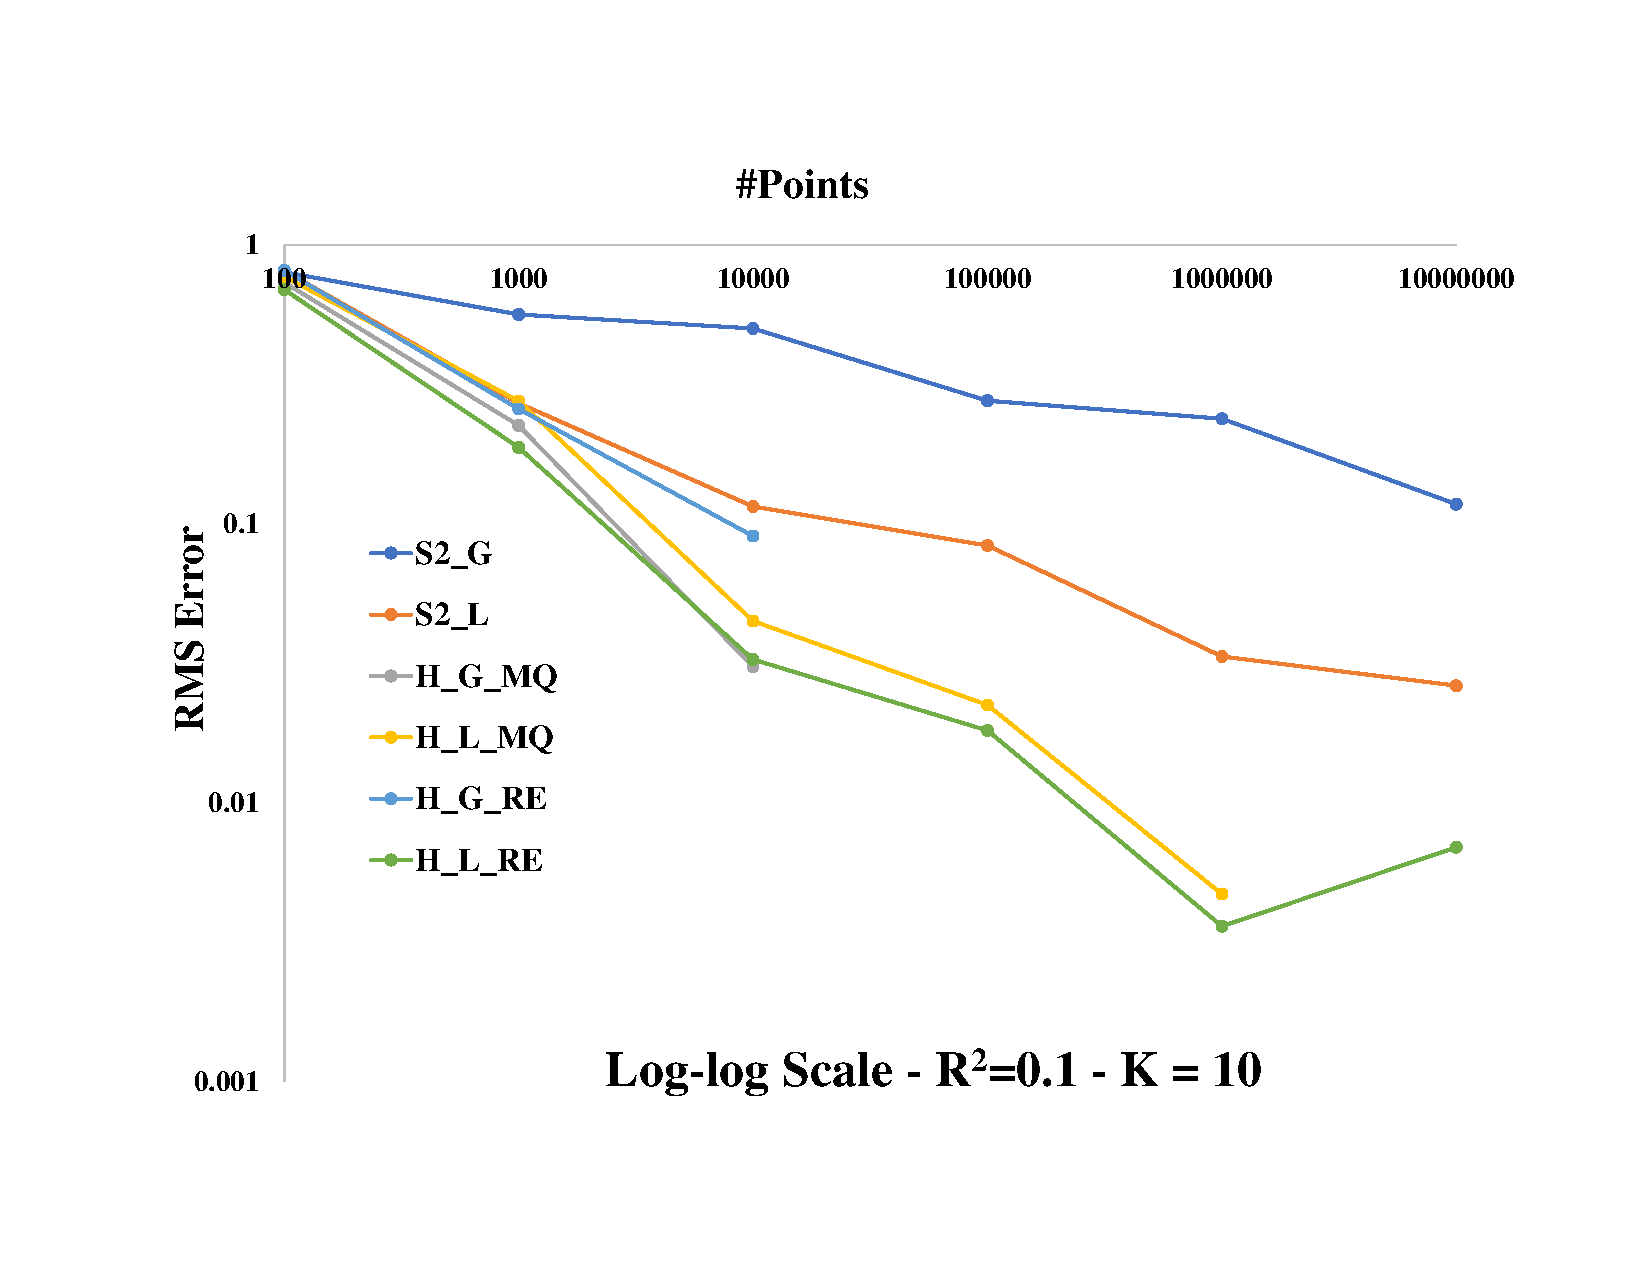
\includegraphics[width=0.49\textwidth]{../viz/points_error.pdf}}
   \subfloat {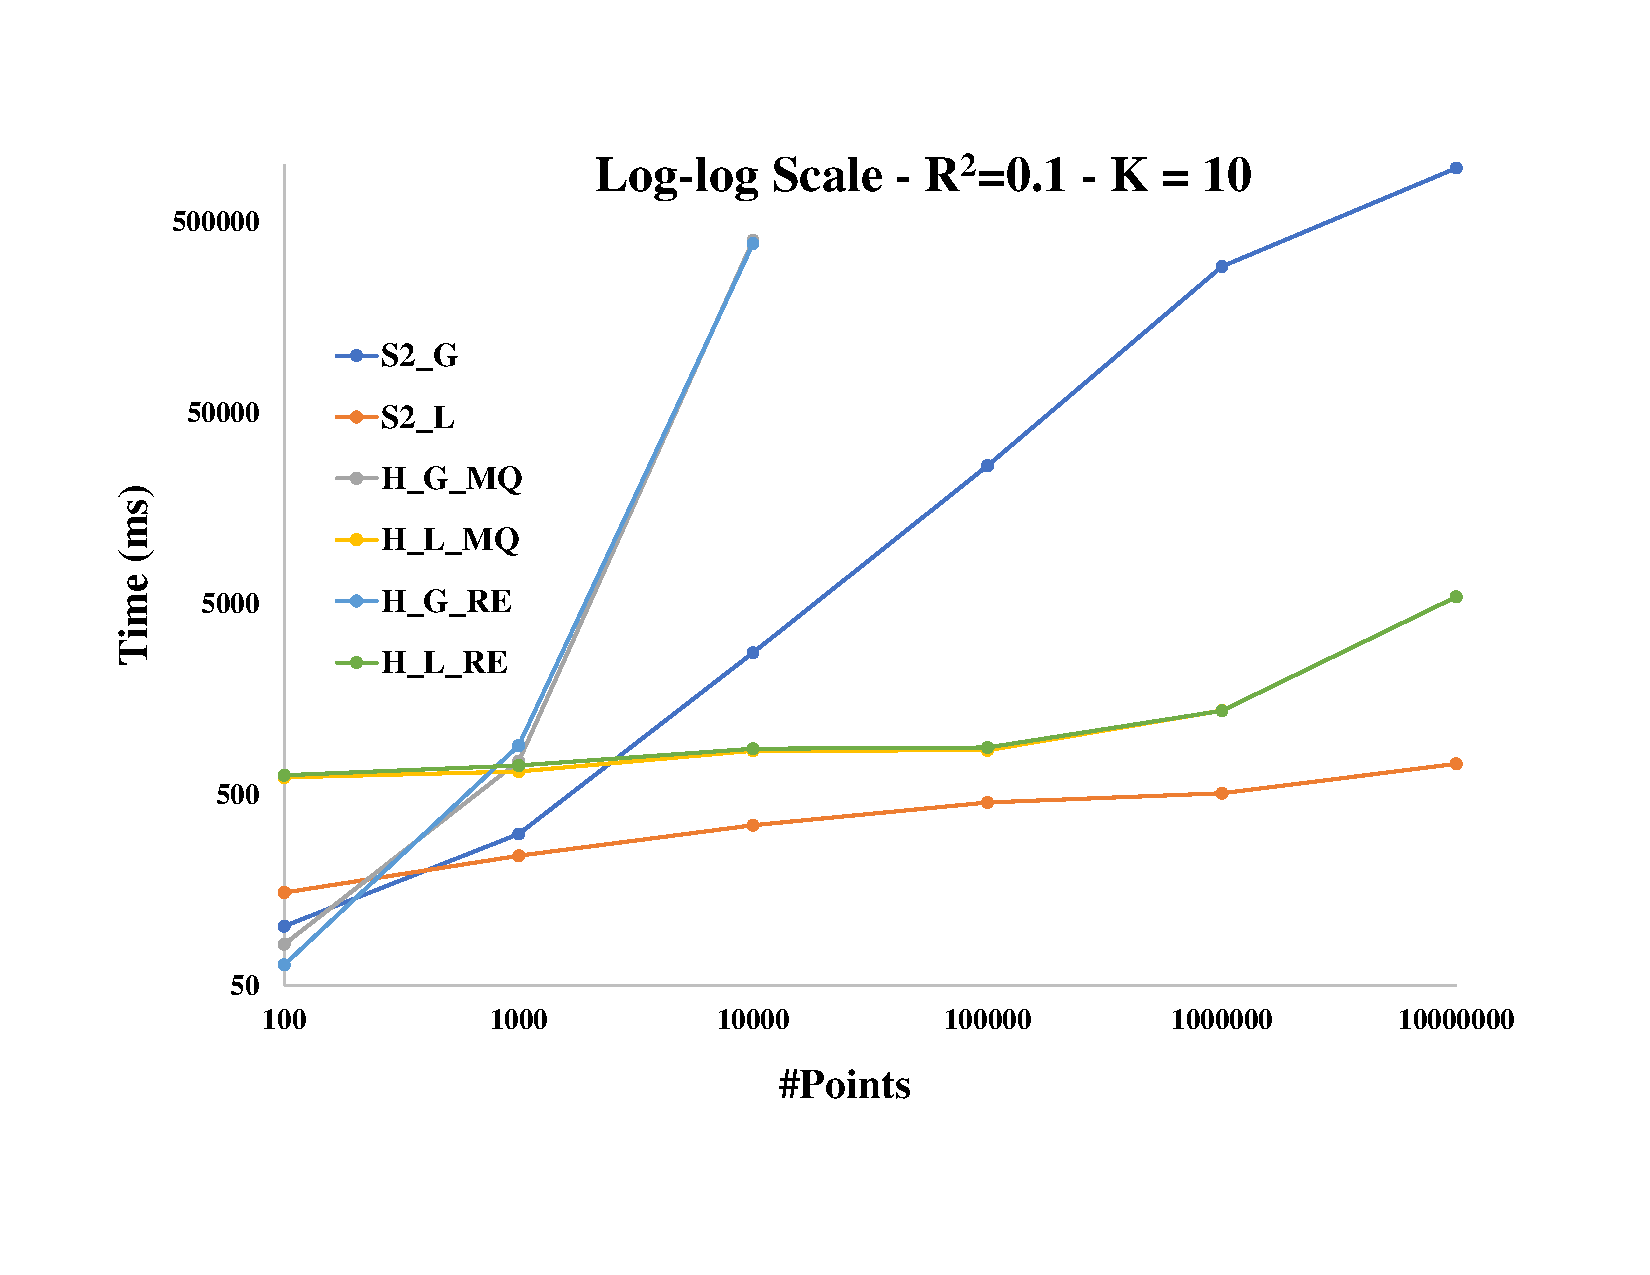
\includegraphics[width=0.49\textwidth]{../viz/points_time.pdf}}   
   \caption{The affect of increasing the number of the scatter data points. Here $K=10$ and $R^{2} = 0.1$.}
   \label{fig:points1}
\end{figure}   
   	    
\begin{figure}[!tbh]
\centering        
  \subfloat {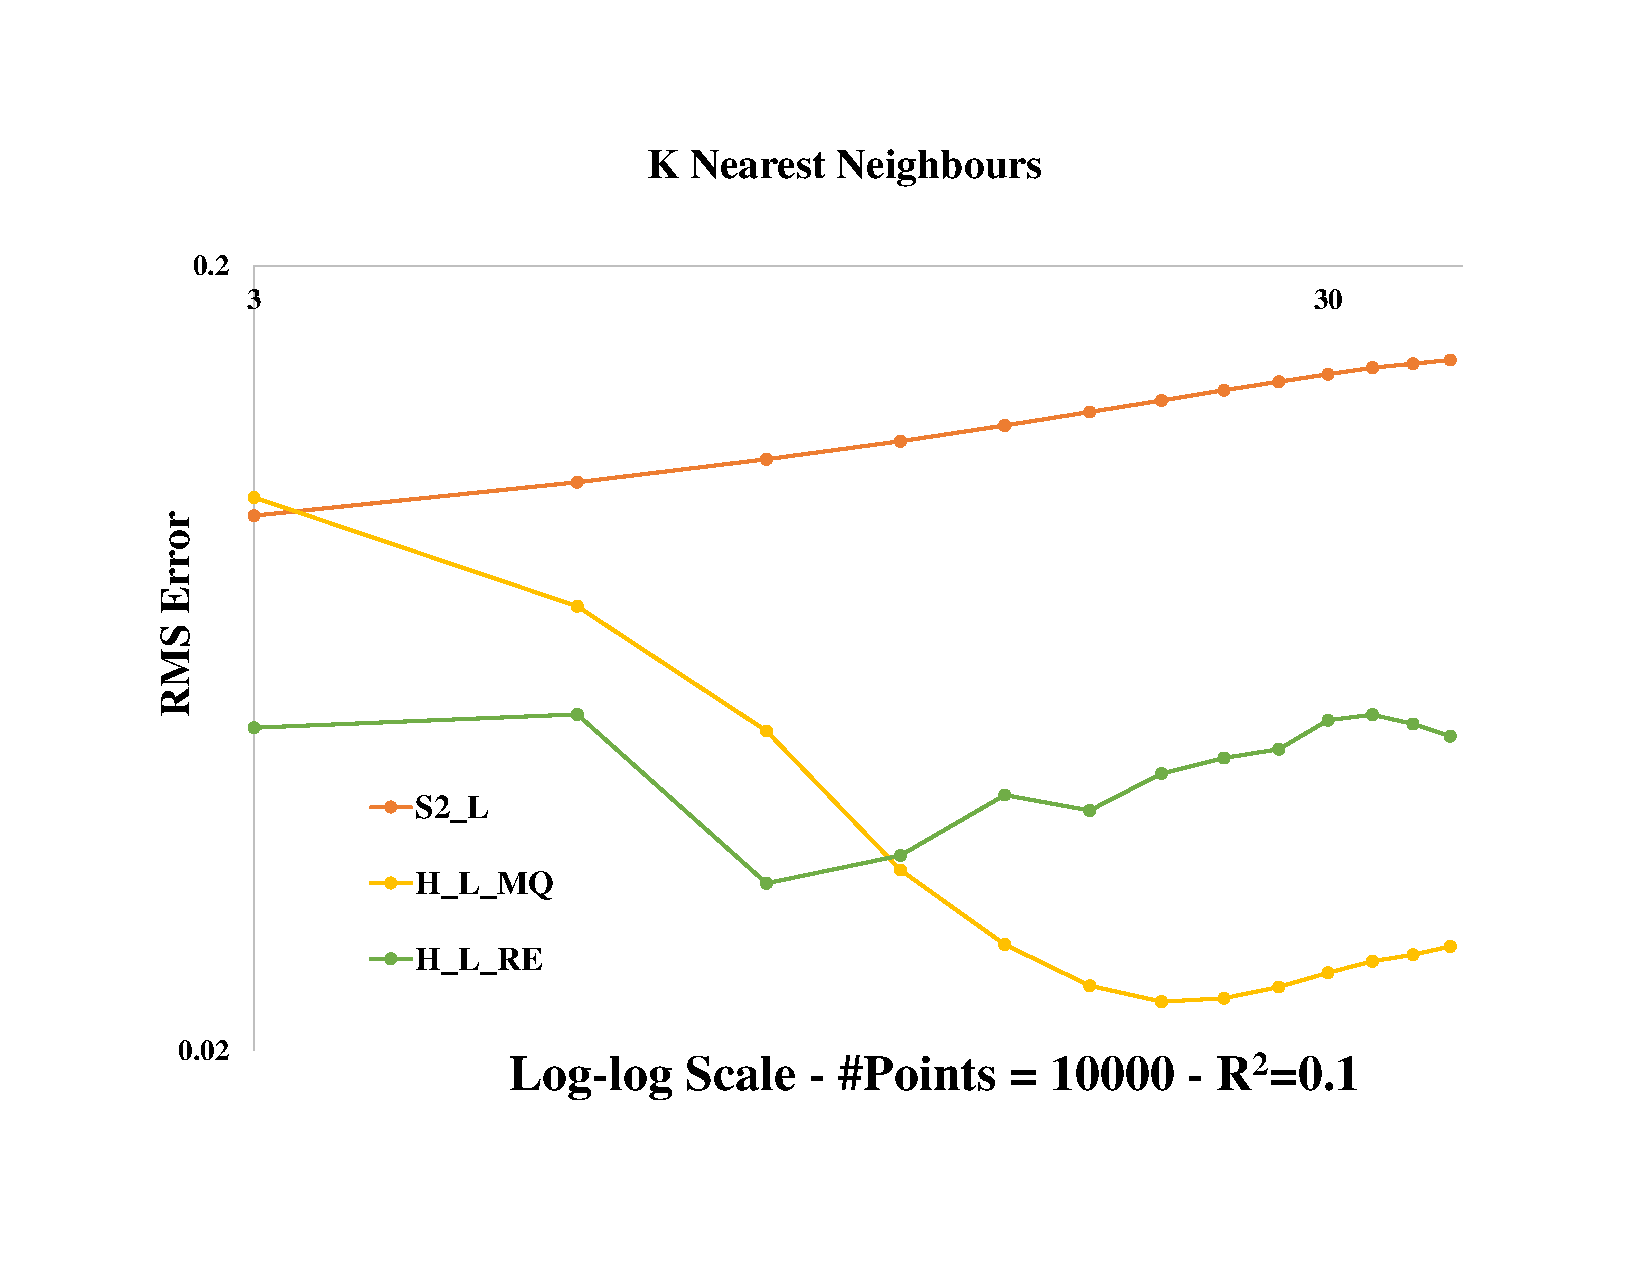
\includegraphics[width=0.49\textwidth]{../viz/k_error.pdf}}
  \subfloat {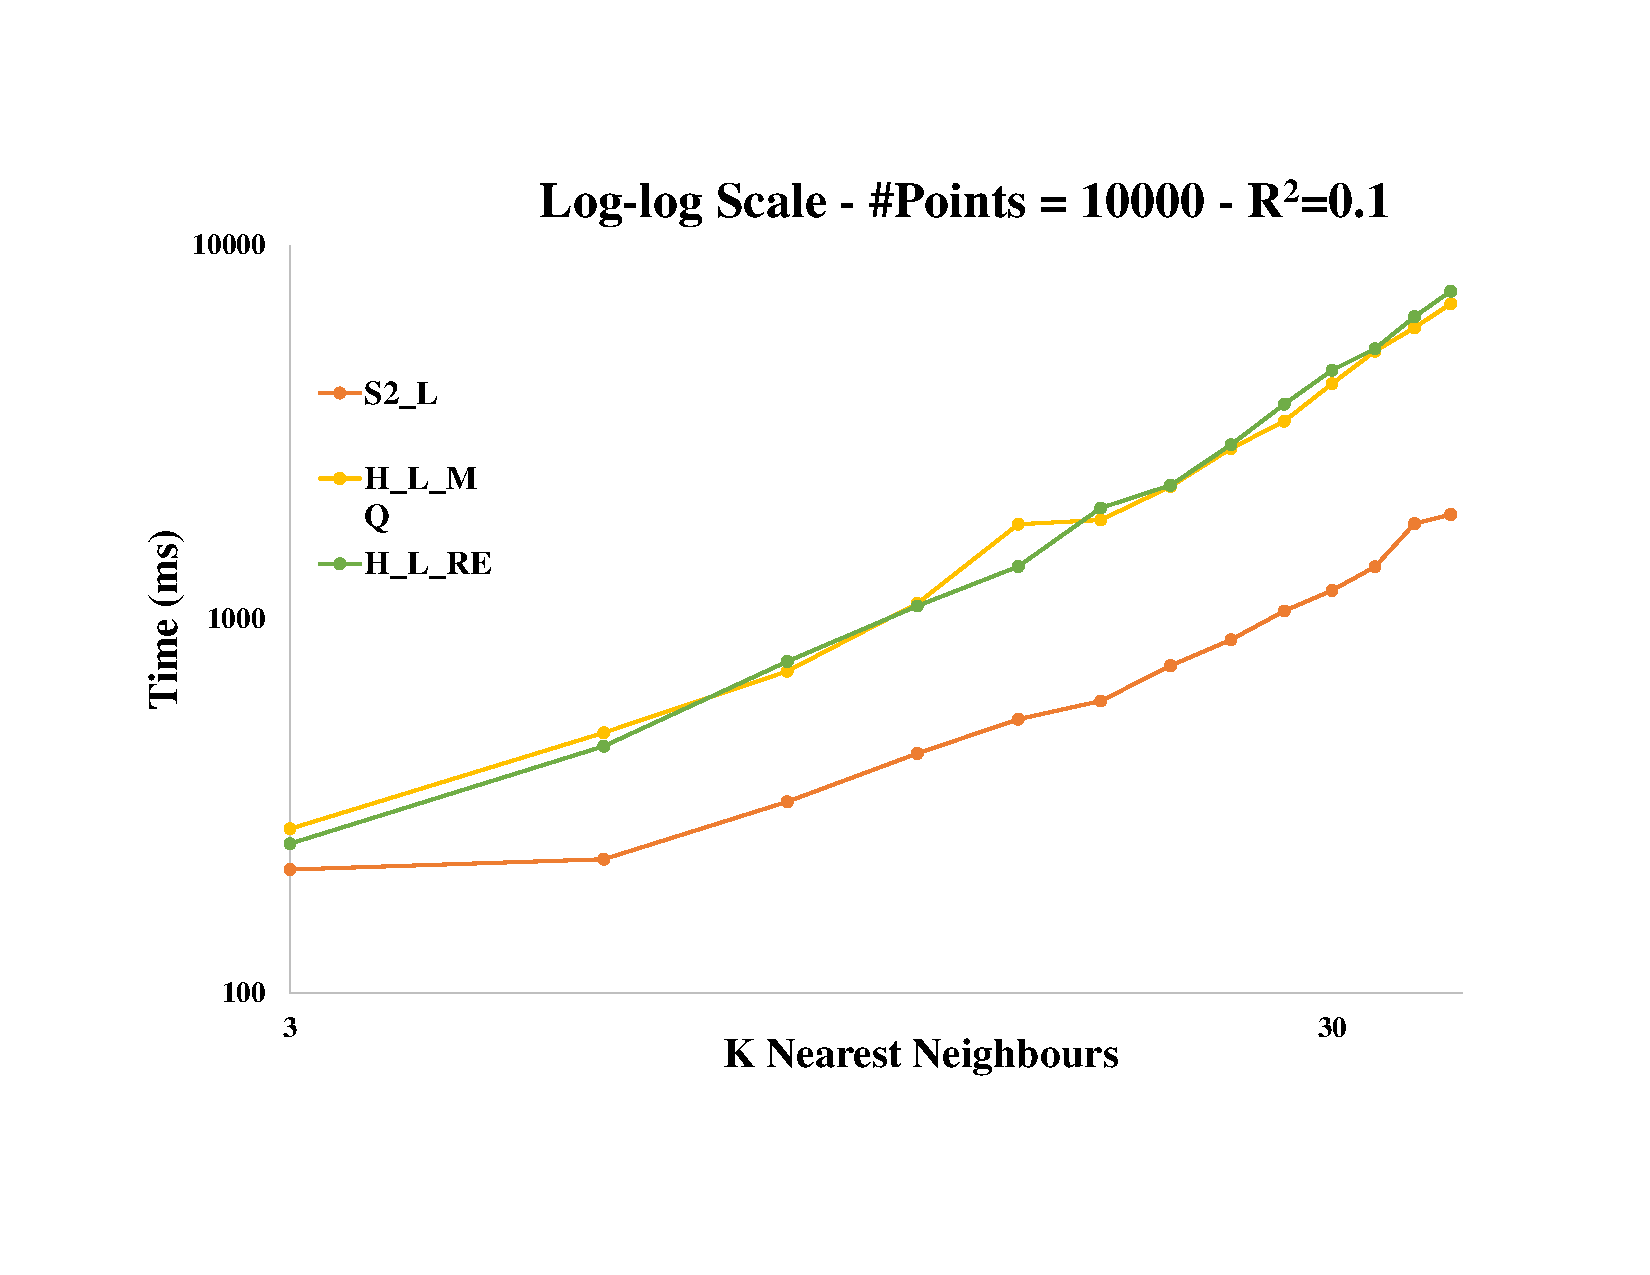
\includegraphics[width=0.49\textwidth]{../viz/k_time.pdf}}
   \caption{The affect of changing the number of K nearest neighbors for local method. Here we used 10000 points with $R^{2}=0.1$.}
   \label{fig:k1}
\end{figure} 	 	        


\begin{figure}[!tbh]
\centering        
   \subfloat {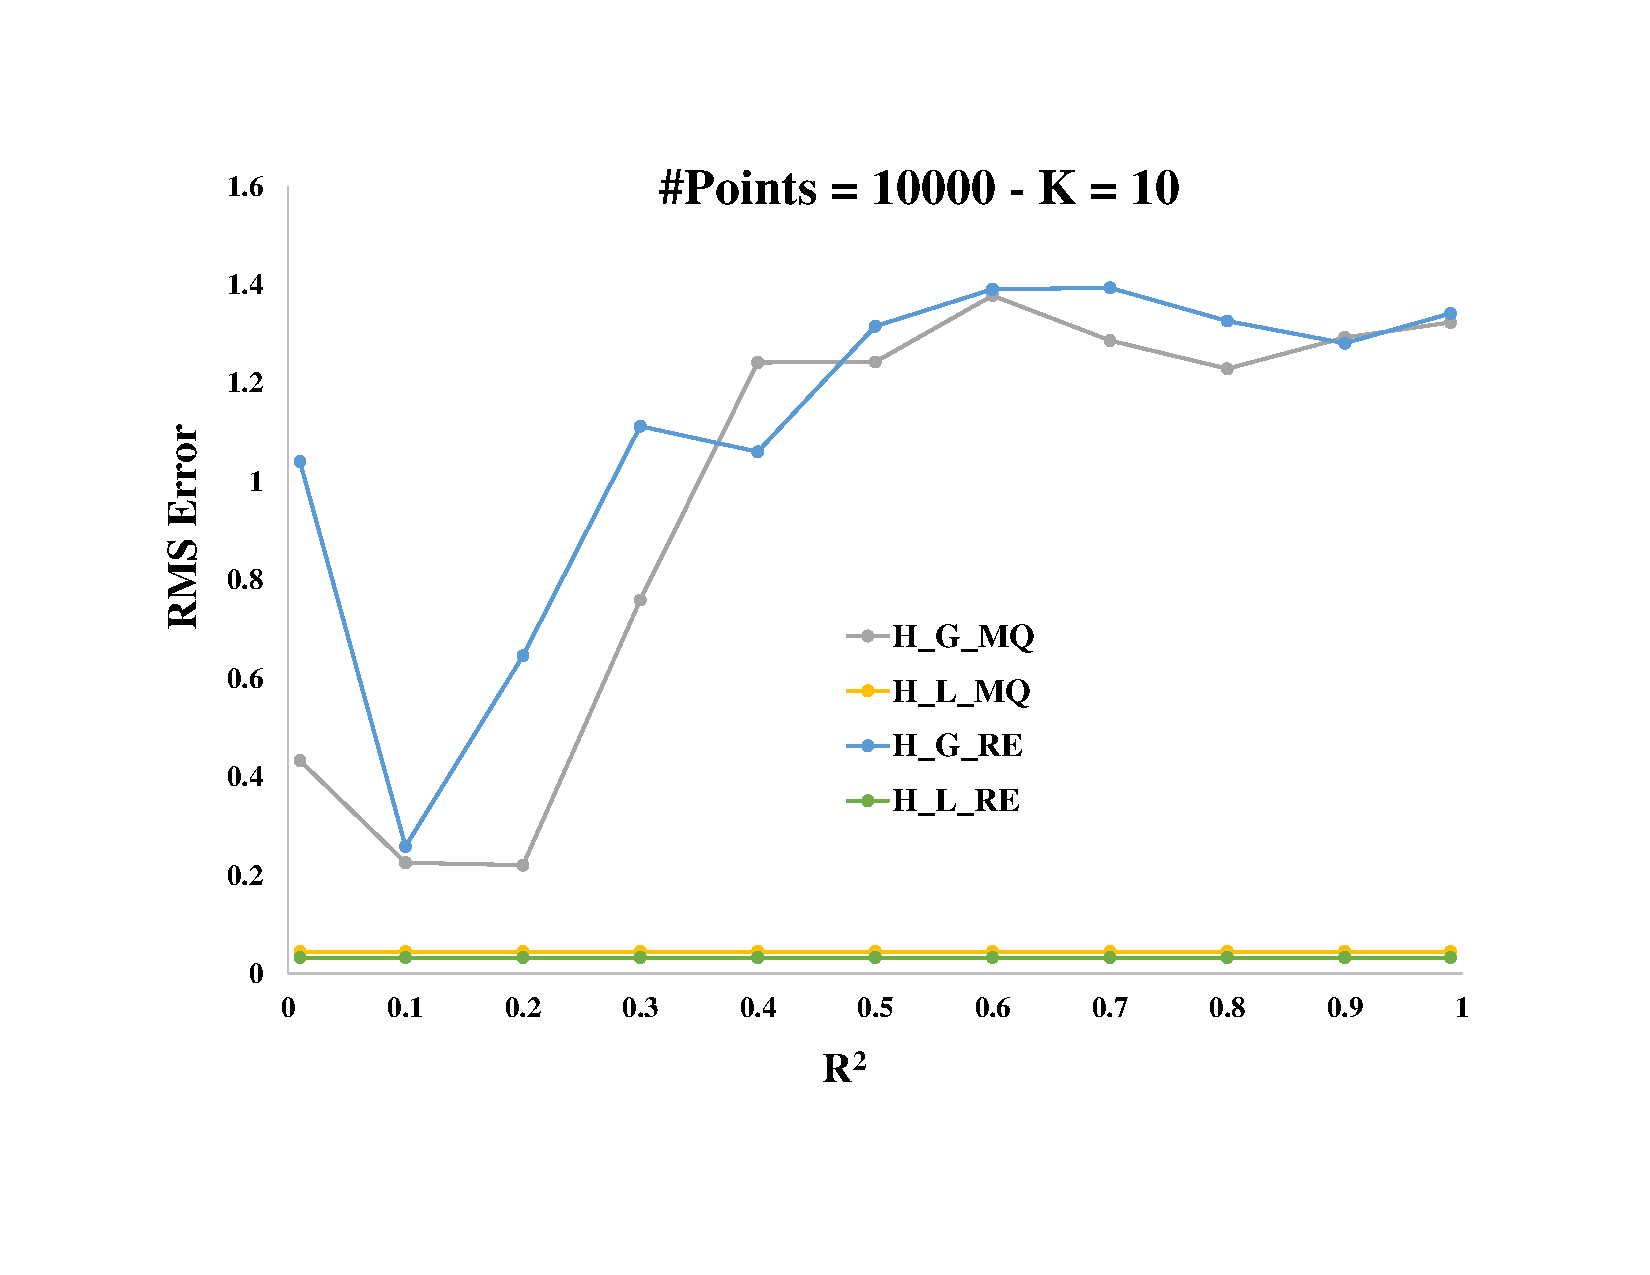
\includegraphics[width=0.46\textwidth]{../viz/r2_error.pdf}}
   \subfloat [Ground Truth] {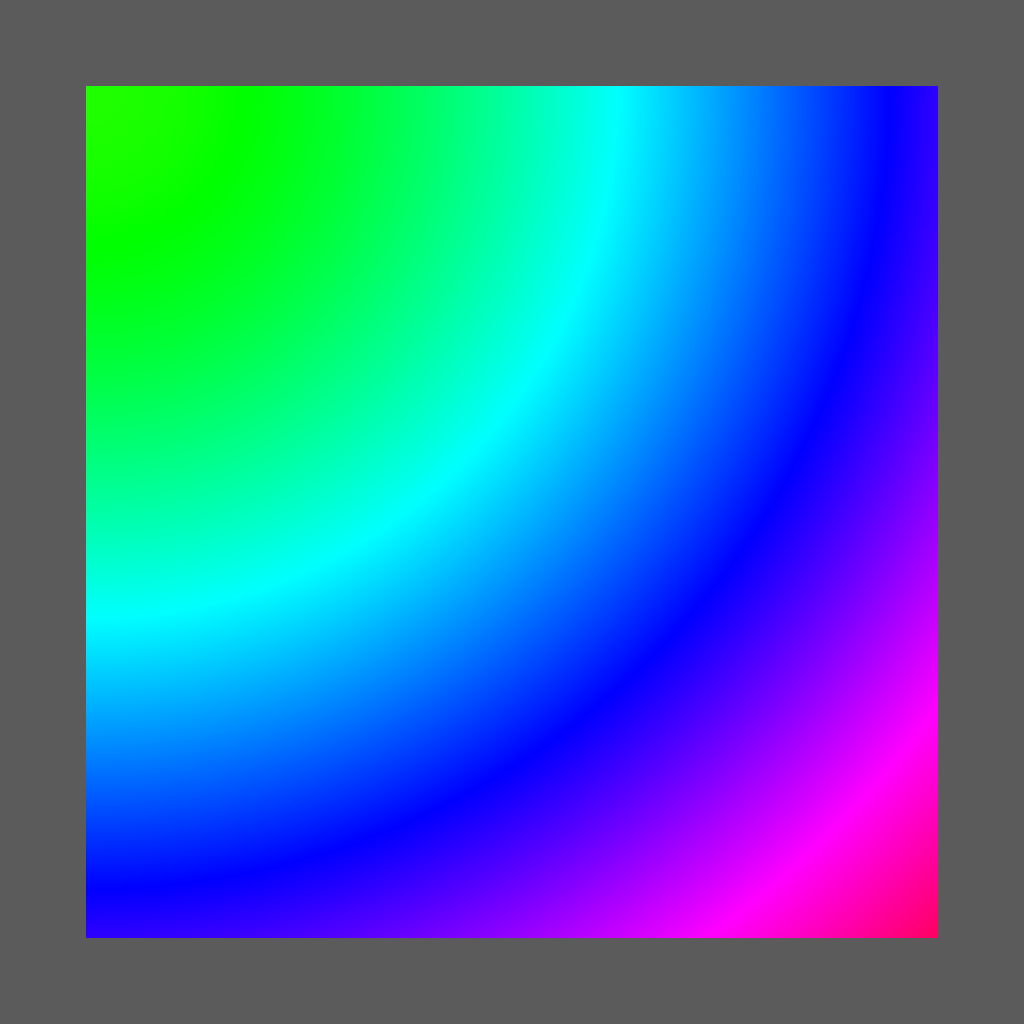
\includegraphics[width=0.30\textwidth]{../viz/ground_truth.png}}
   \caption{The affect of $R^{2}$ factor in Hardy's methods. Here we used 10000 points with $K=10$.}
   \label{fig:r21}
\end{figure} 	    
	        
%======================================================	                
	        	        
\newpage
\begin{figure}[!tbh]
\centering        
   \rotatebox[origin=l]{90}{G Shepard's 2}	
   \subfloat [100] {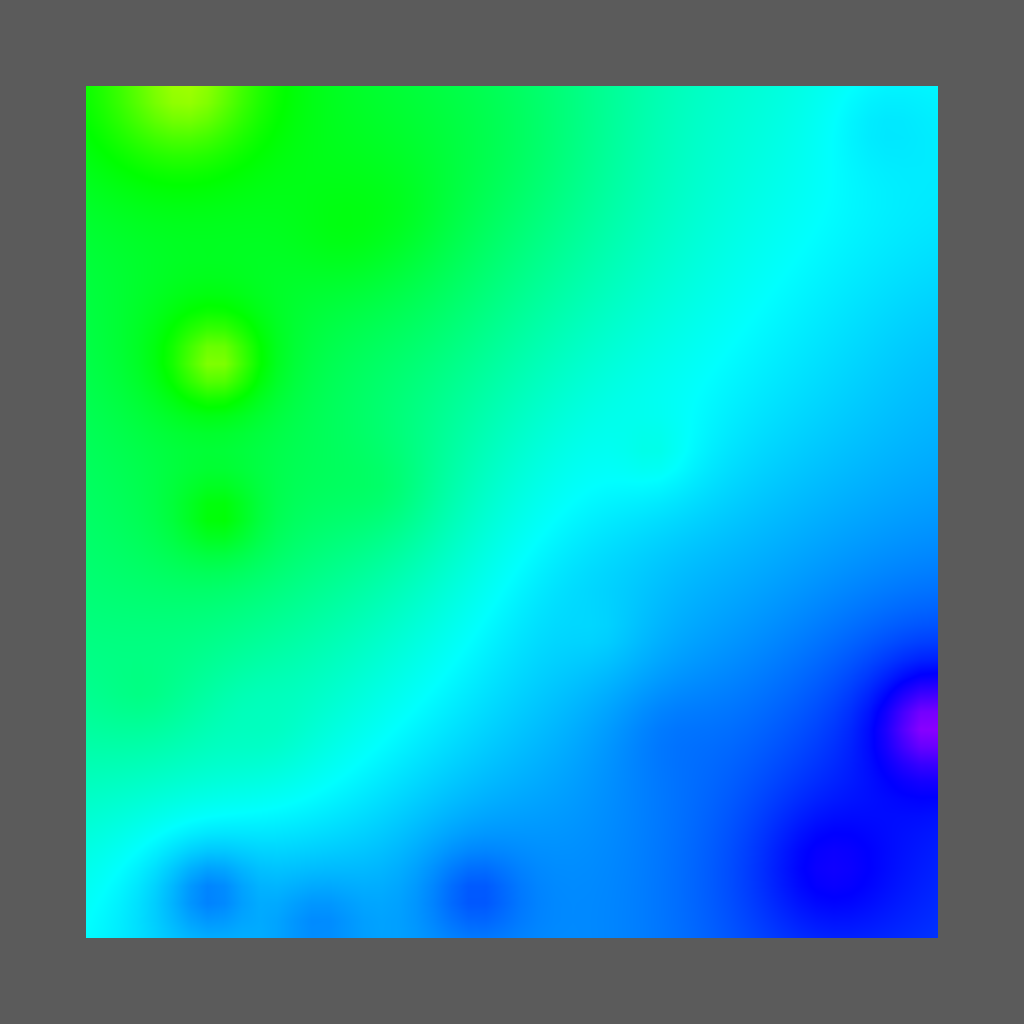
\includegraphics[width=0.16\textwidth]{../viz/num_points/S2_G/100_spheres_S2_G.png}}
   \subfloat [1000] {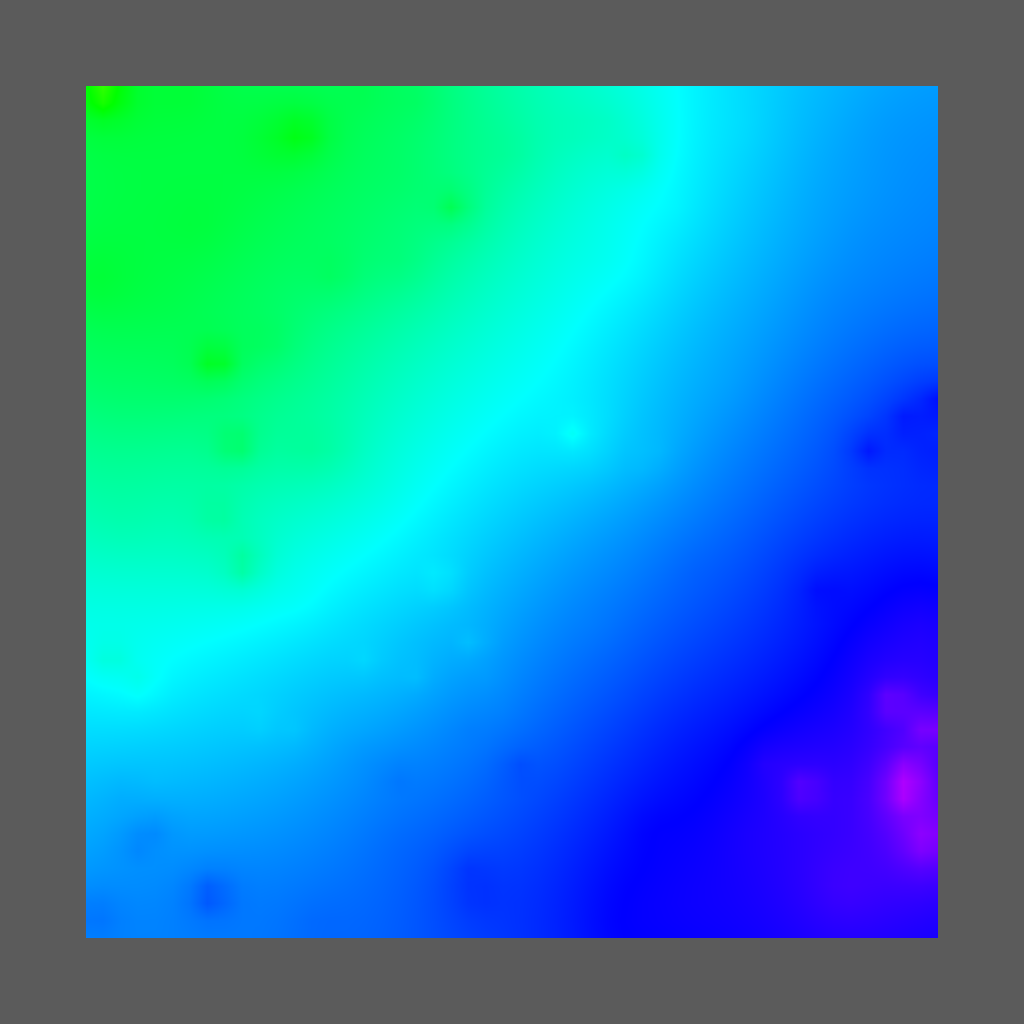
\includegraphics[width=0.16\textwidth]{../viz/num_points/S2_G/1000_spheres_S2_G.png}}
   \subfloat [10000] {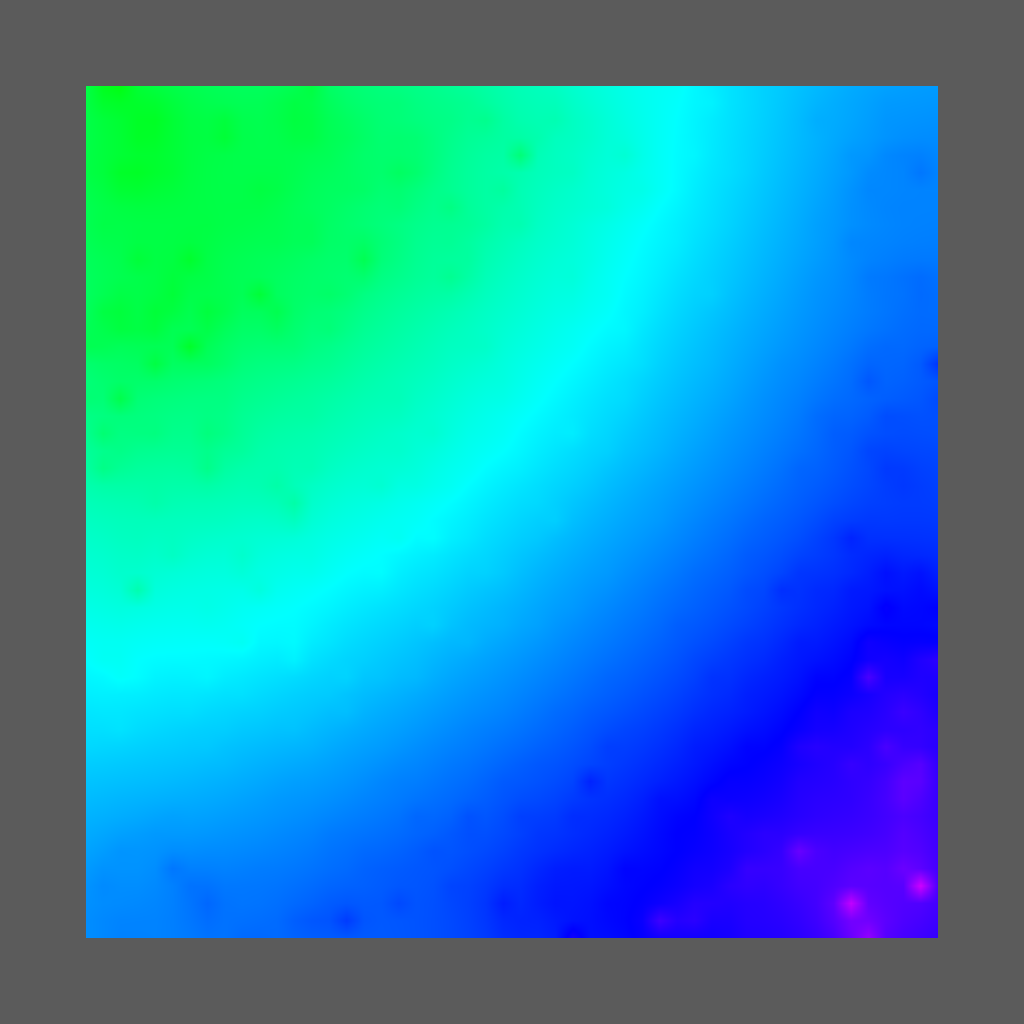
\includegraphics[width=0.16\textwidth]{../viz/num_points/S2_G/10000_spheres_S2_G.png}}
   \subfloat [100000] {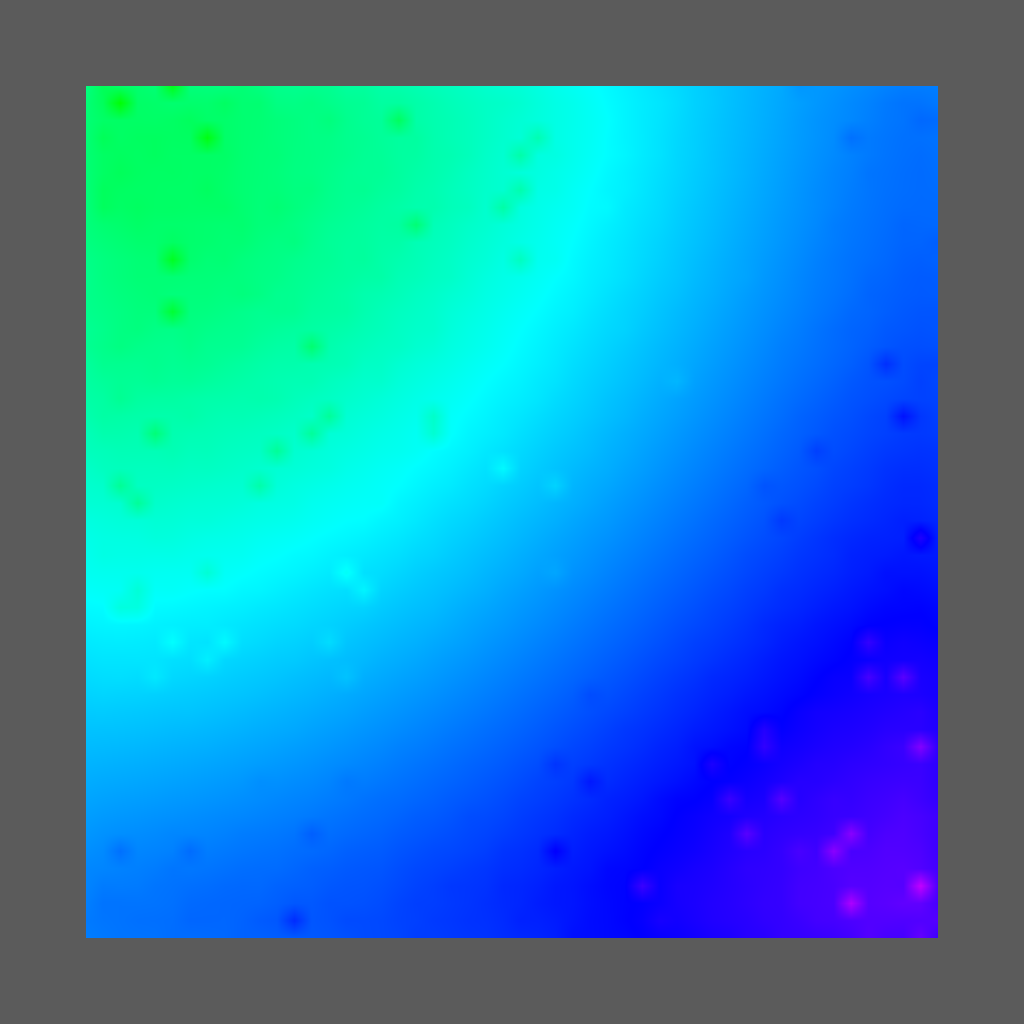
\includegraphics[width=0.16\textwidth]{../viz/num_points/S2_G/100000_spheres_S2_G.png}}
   \subfloat [1000000] {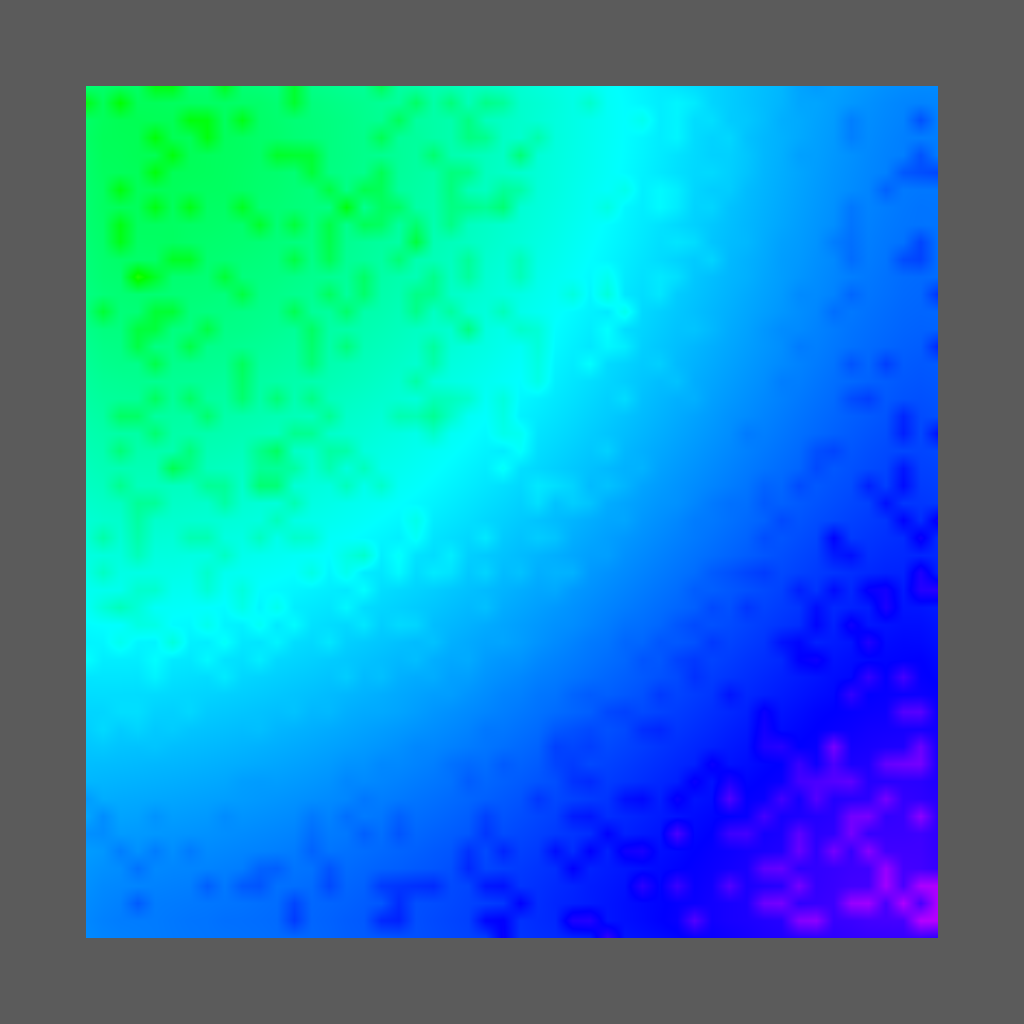
\includegraphics[width=0.16\textwidth]{../viz/num_points/S2_G/1000000_spheres_S2_G.png}}
   \subfloat [10000000] {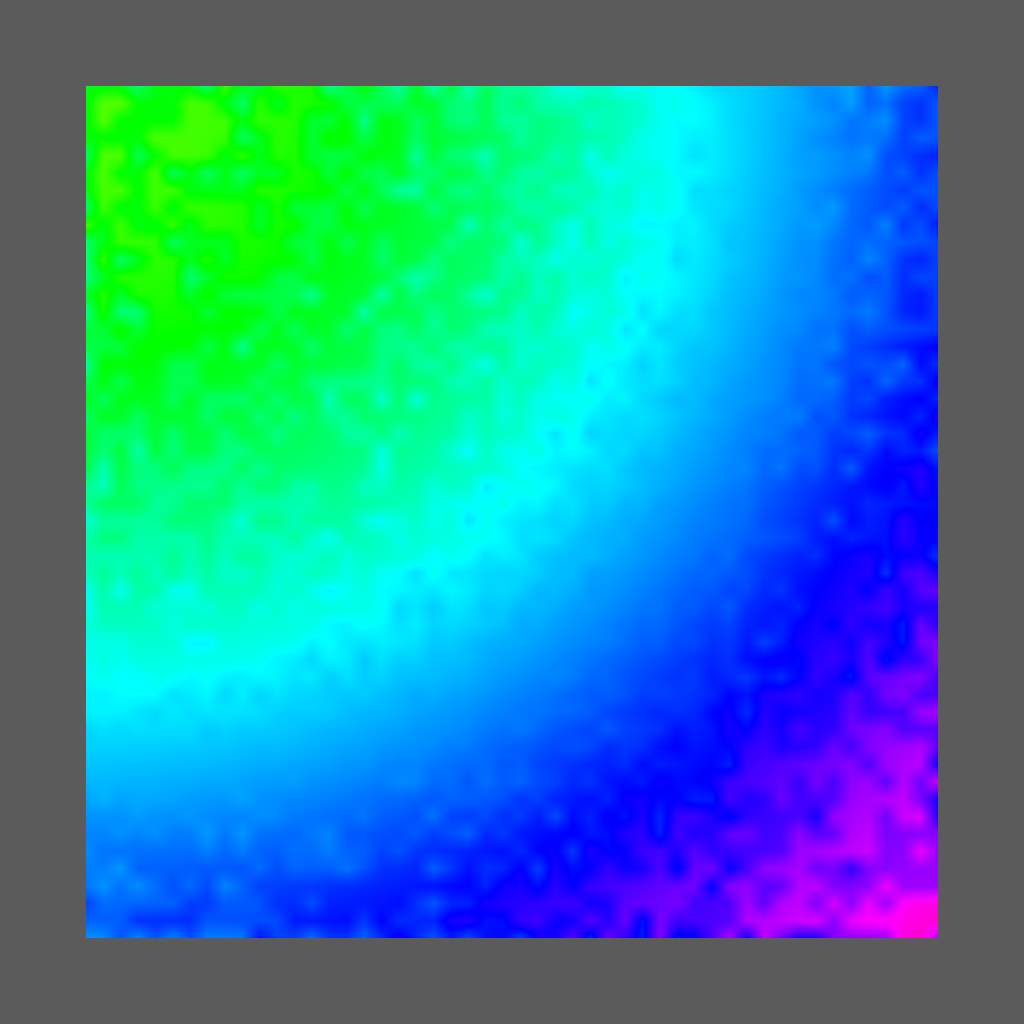
\includegraphics[width=0.16\textwidth]{../viz/num_points/S2_G/10000000_spheres_S2_G.png}}
   
   \rotatebox[origin=l]{90}{L Shepard's 2}	
   \subfloat [100] {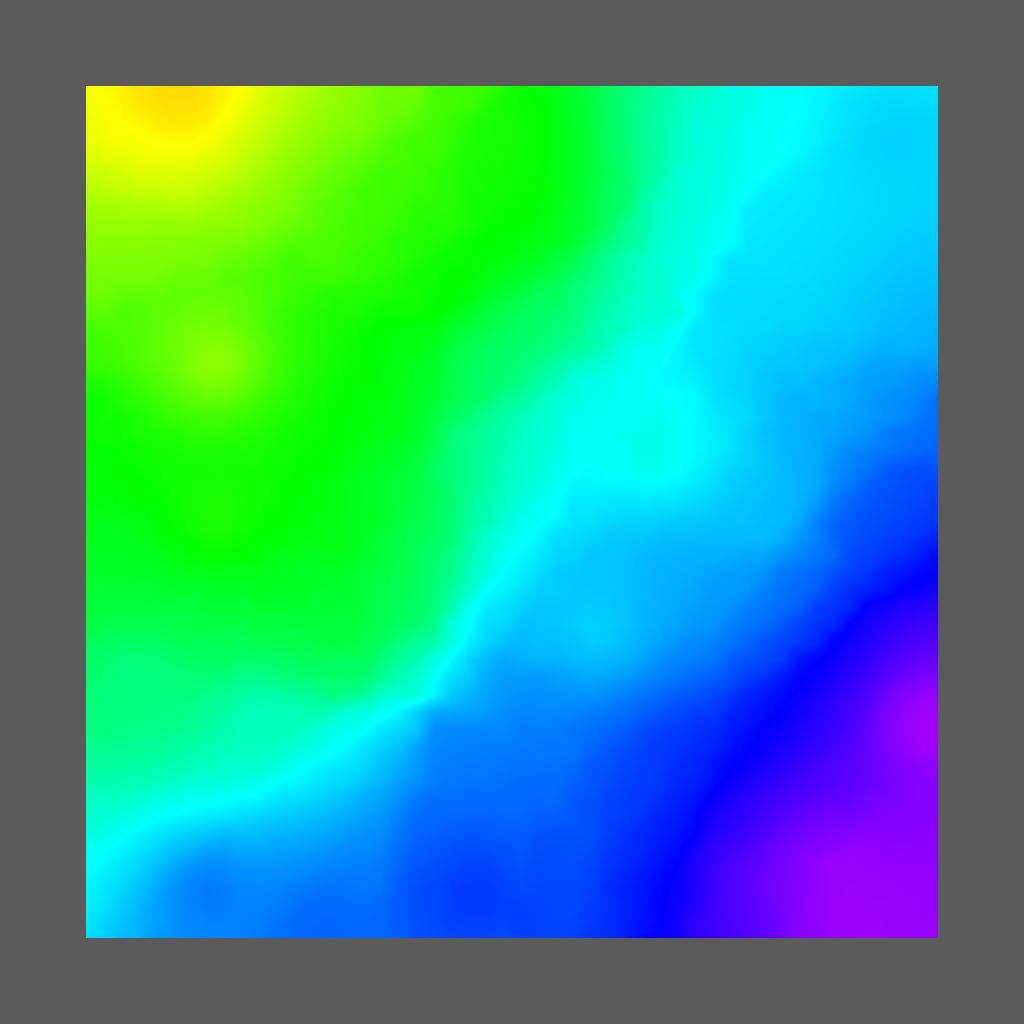
\includegraphics[width=0.16\textwidth]{../viz/num_points/S2_L/100_spheres_S2_L.png}}
   \subfloat [1000] {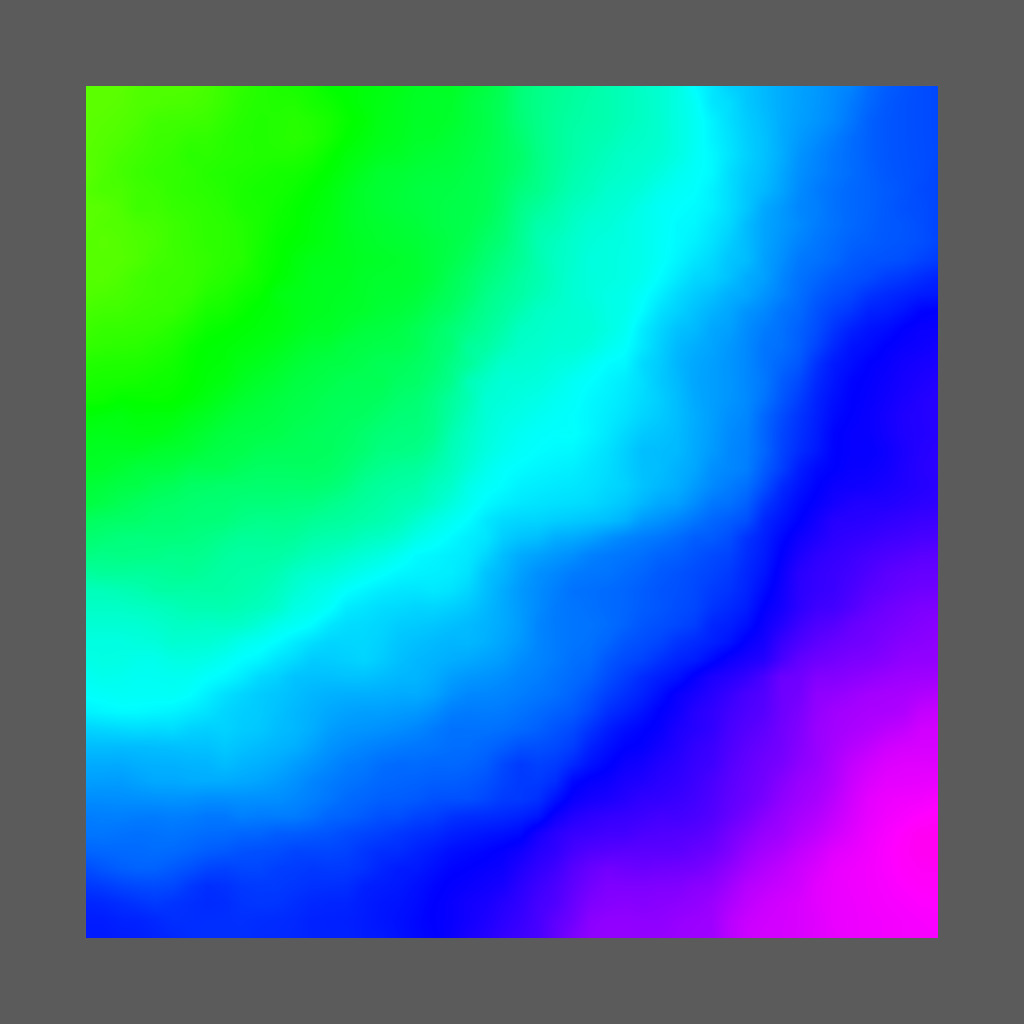
\includegraphics[width=0.16\textwidth]{../viz/num_points/S2_L/1000_spheres_S2_L.png}}
   \subfloat [10000] {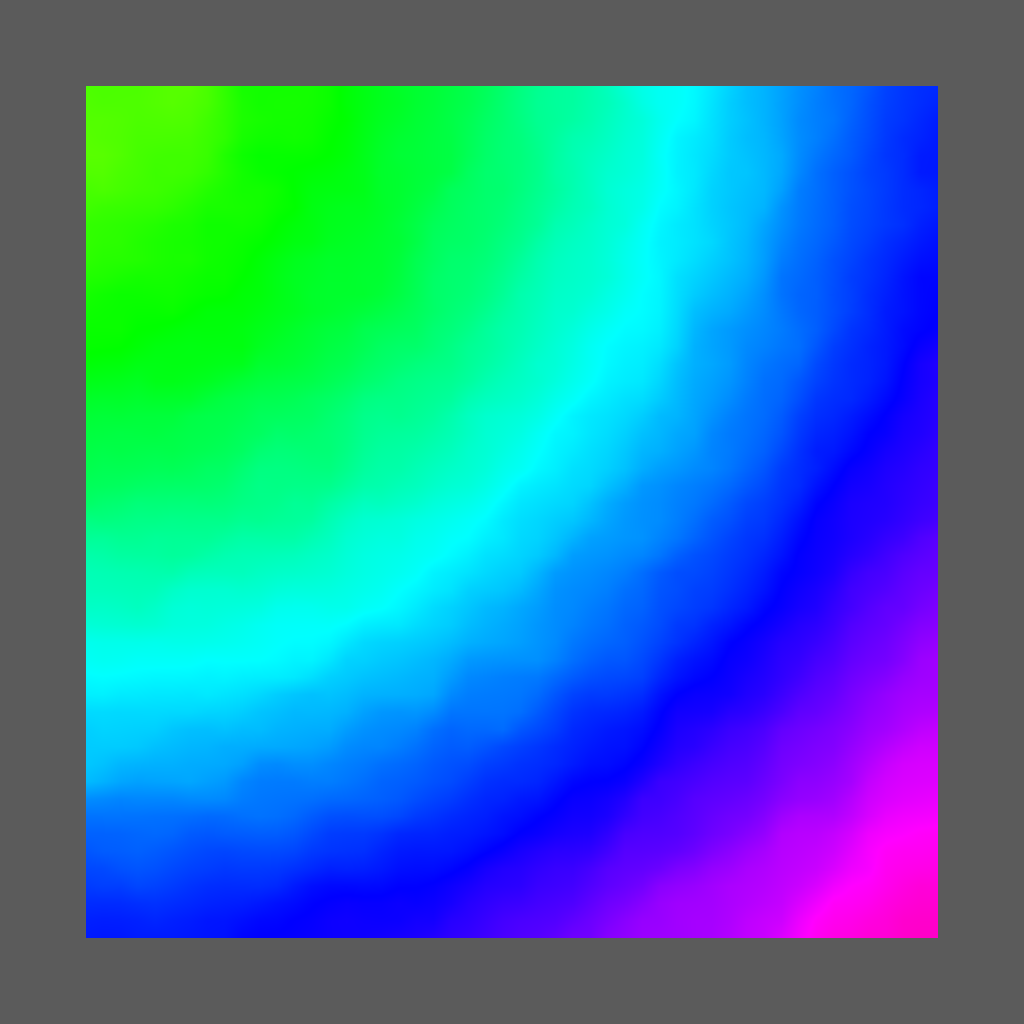
\includegraphics[width=0.16\textwidth]{../viz/num_points/S2_L/10000_spheres_S2_L.png}}
   \subfloat [100000] {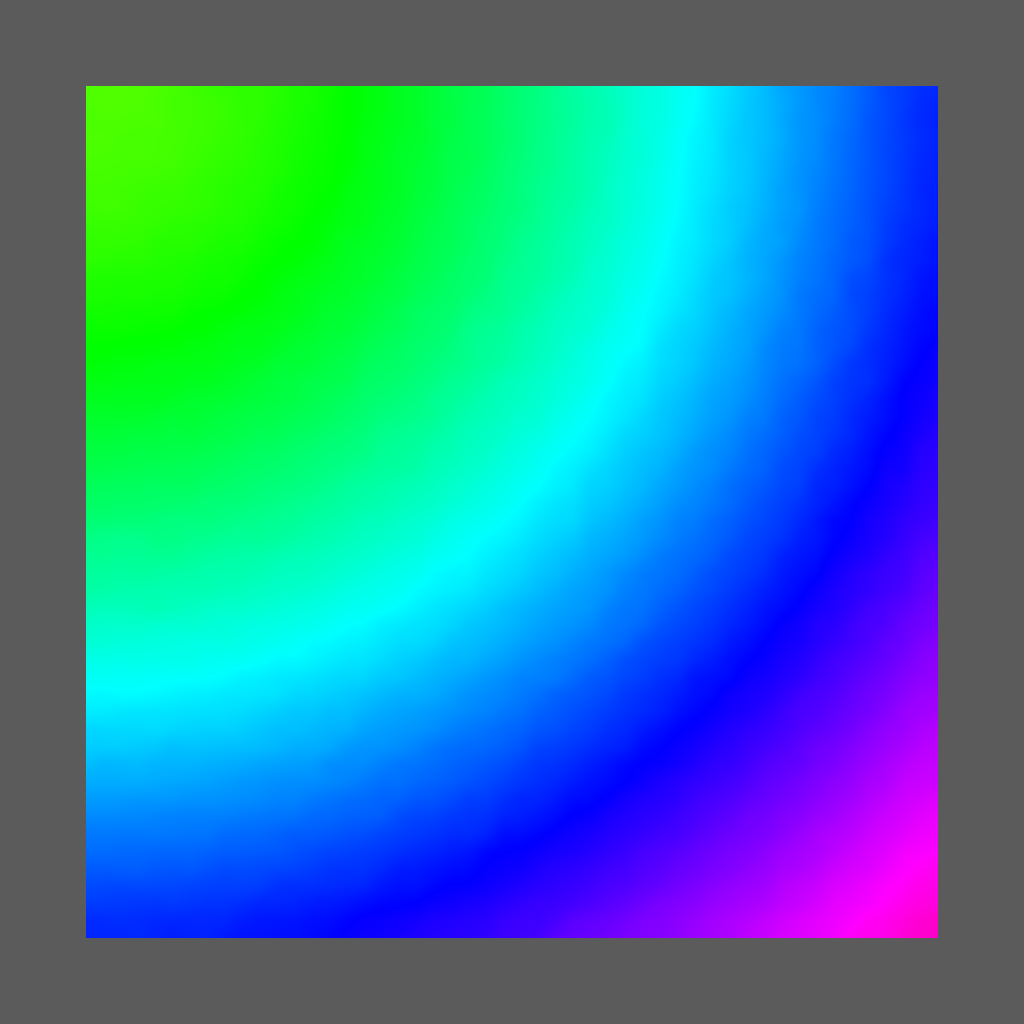
\includegraphics[width=0.16\textwidth]{../viz/num_points/S2_L/100000_spheres_S2_L.png}}
   \subfloat [1000000] {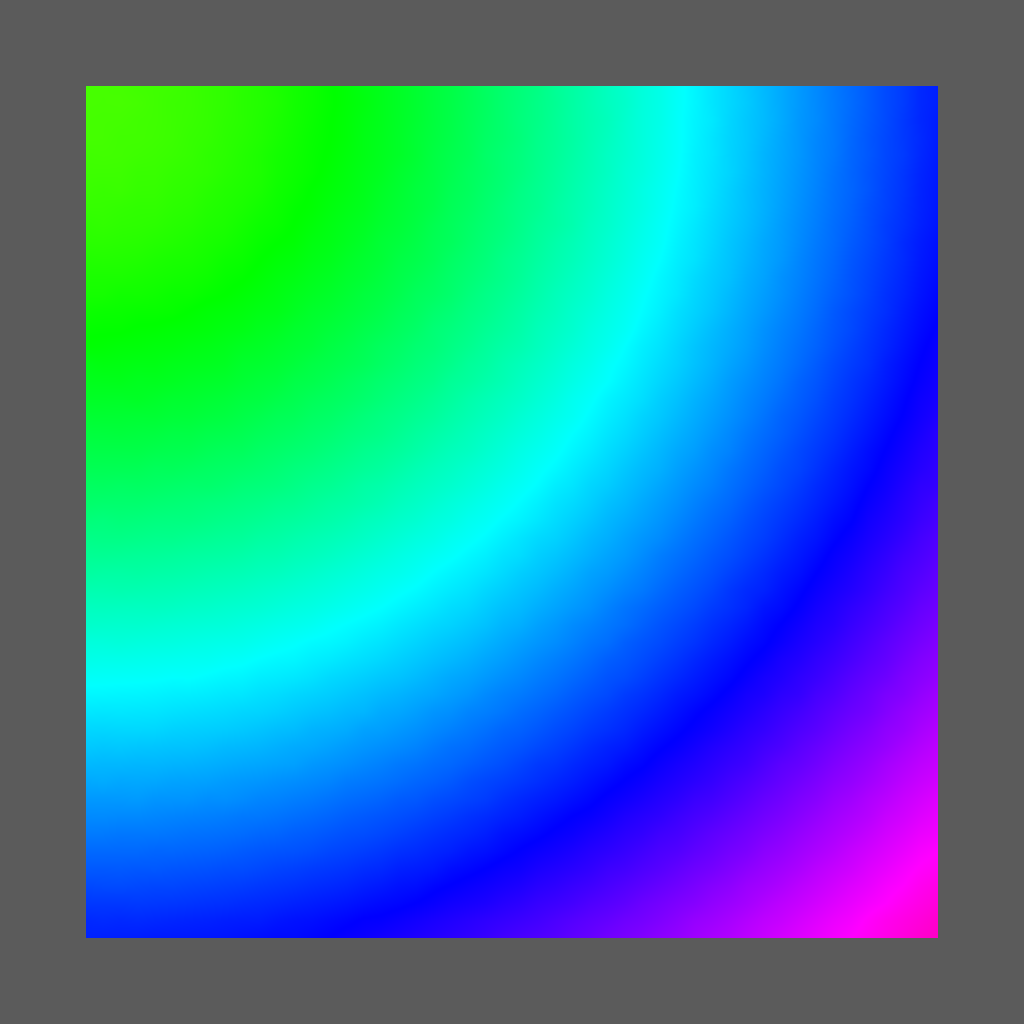
\includegraphics[width=0.16\textwidth]{../viz/num_points/S2_L/1000000_spheres_S2_L.png}}
   \subfloat [10000000] {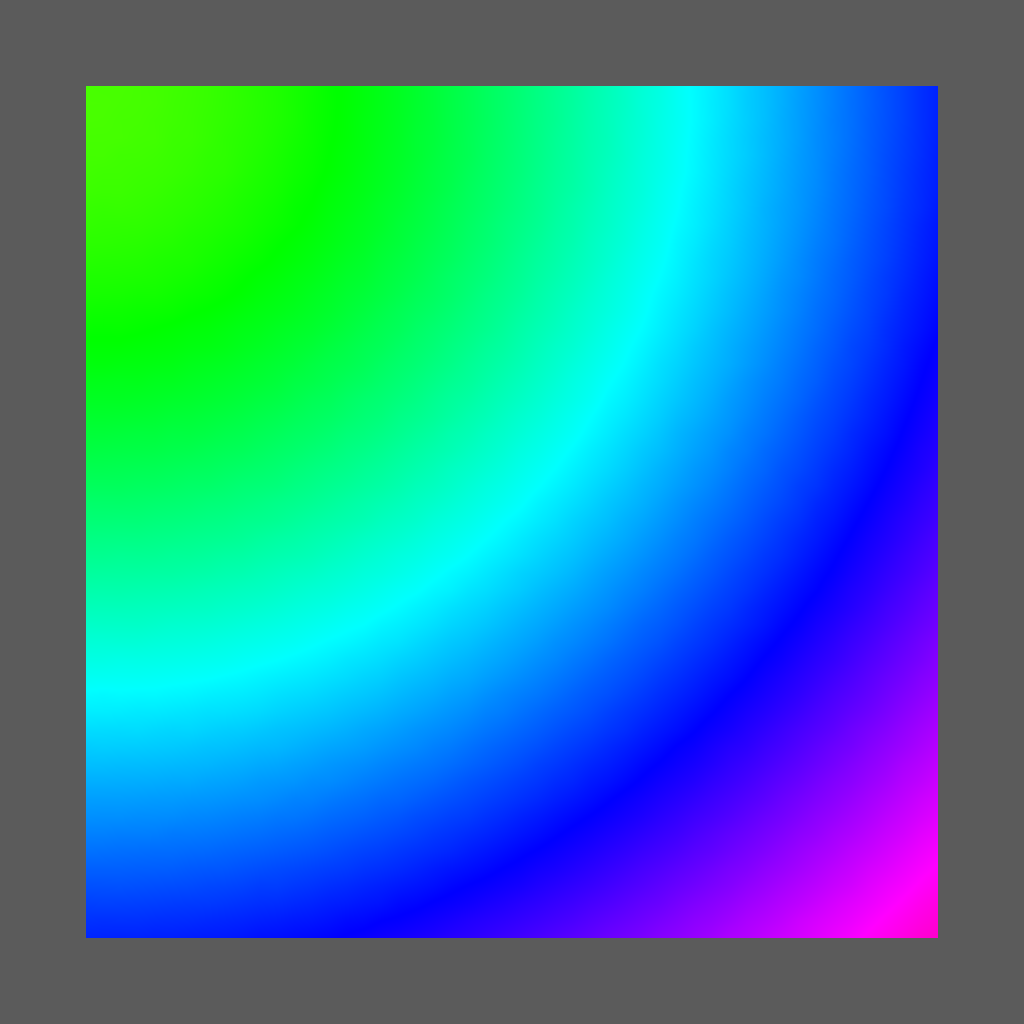
\includegraphics[width=0.16\textwidth]{../viz/num_points/S2_L/10000000_spheres_S2_L.png}}
   
   \rotatebox[origin=l]{90}{G Hardy MQ}	
   \subfloat [100] {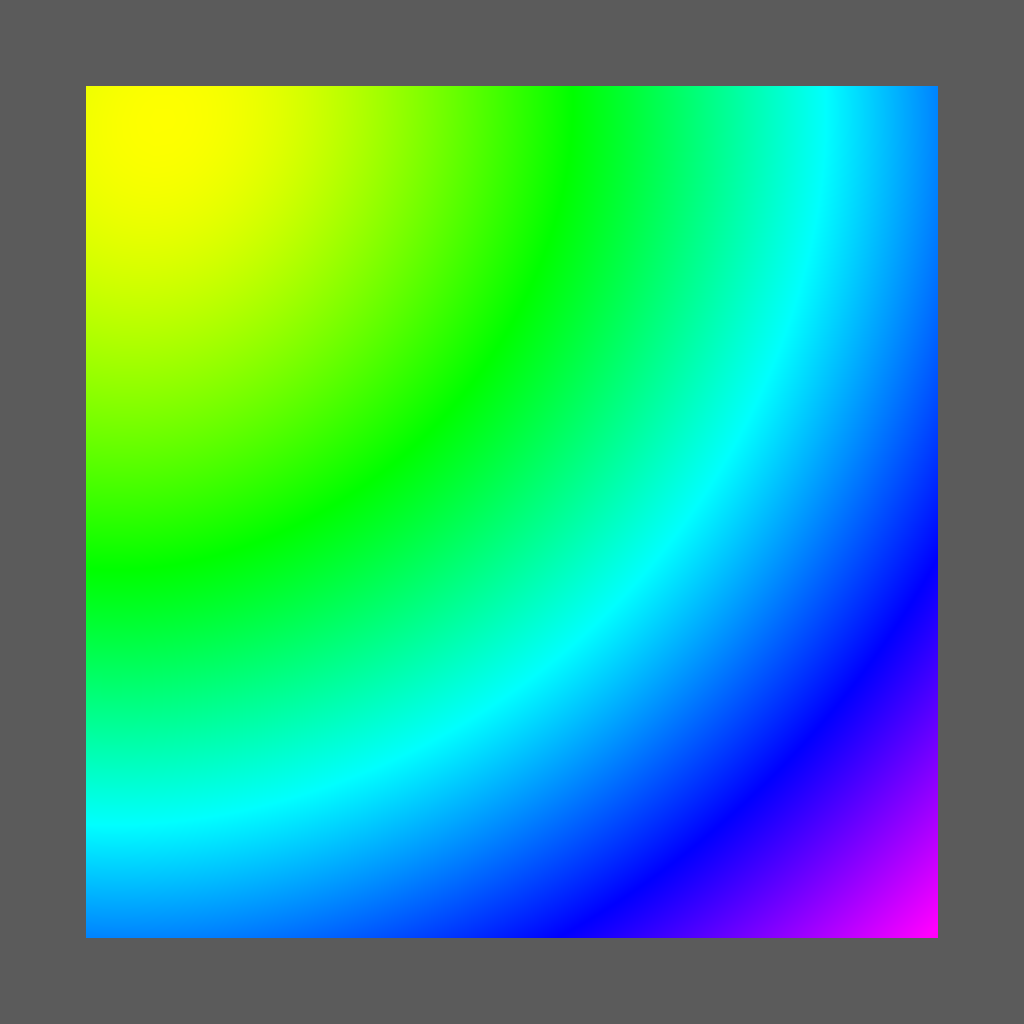
\includegraphics[width=0.16\textwidth]{../viz/num_points/H_G_MQ/100_spheres_H_G_MQ.png}}
   \subfloat [1000] {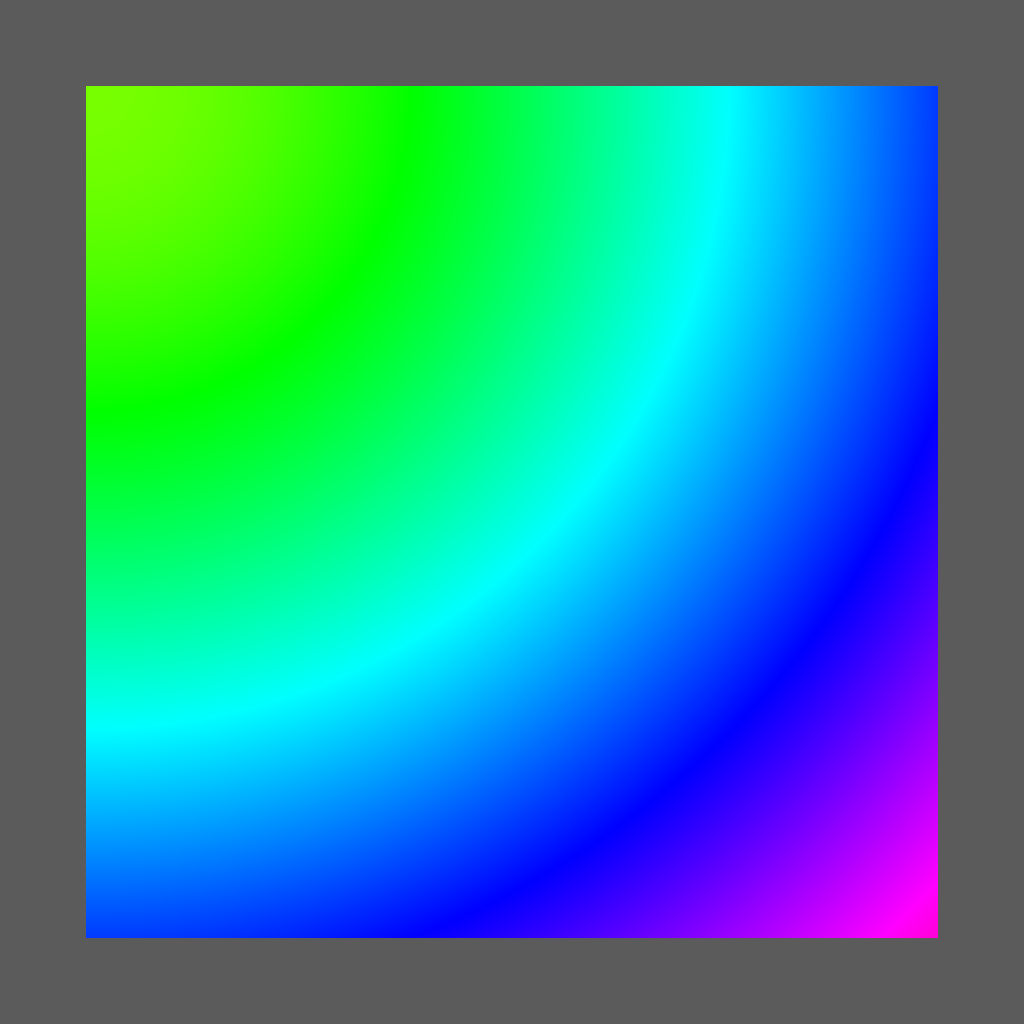
\includegraphics[width=0.16\textwidth]{../viz/num_points/H_G_MQ/1000_spheres_H_G_MQ.png}}
   \subfloat [10000] {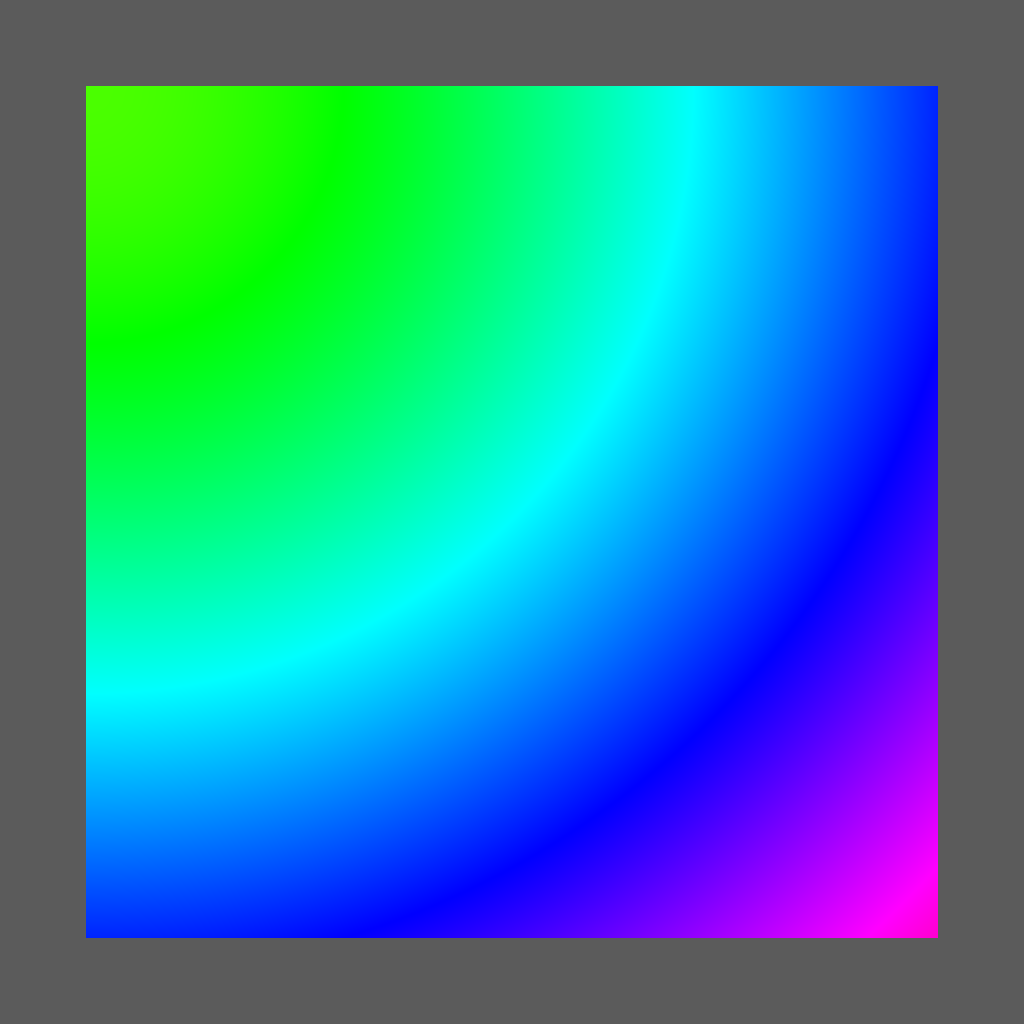
\includegraphics[width=0.16\textwidth]{../viz/num_points/H_G_MQ/10000_spheres_H_G_MQ.png}}
   \subfloat  {
\includegraphics[width=0.16\textwidth]{dummy.png}}
   \subfloat  {
\includegraphics[width=0.16\textwidth]{dummy.png}}
   \subfloat  {
\includegraphics[width=0.16\textwidth]{dummy.png}}   

   \rotatebox[origin=l]{90}{L Hardy MQ}	
   \subfloat [100] {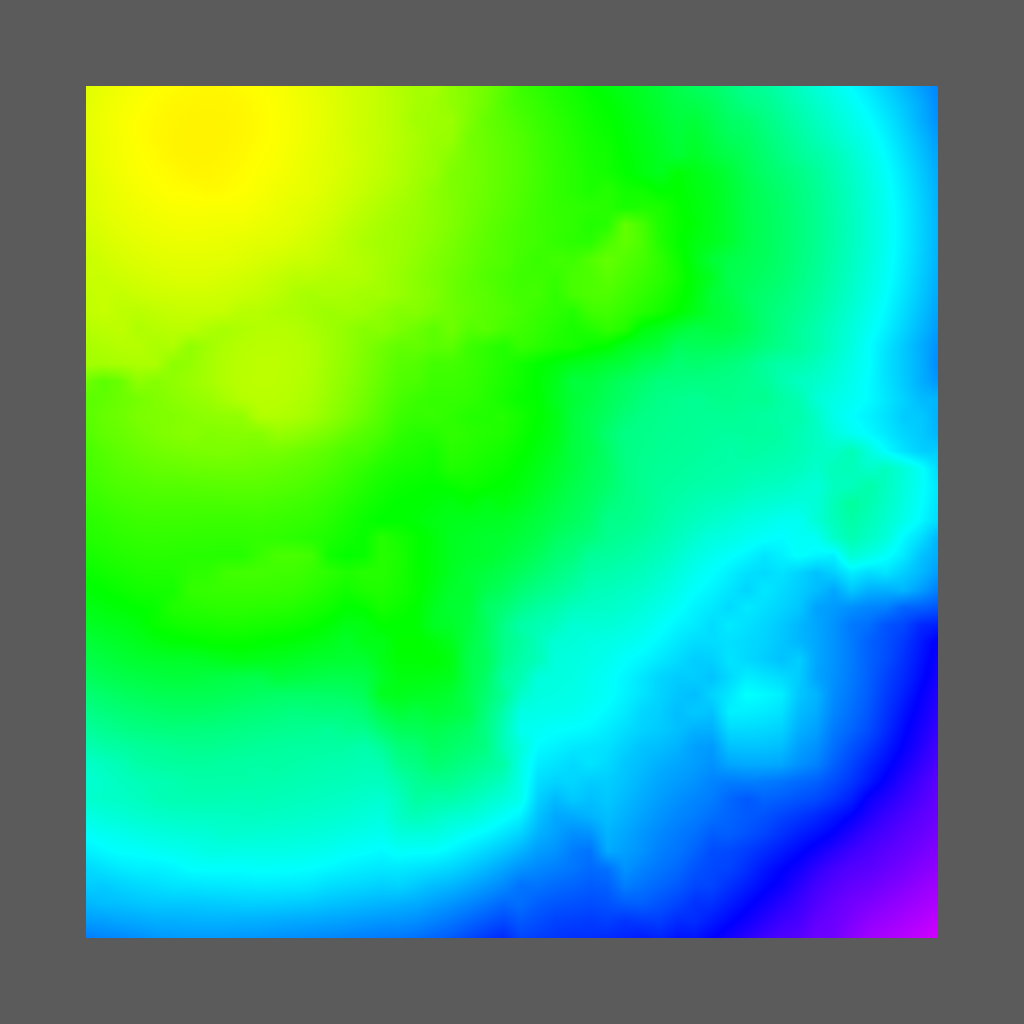
\includegraphics[width=0.16\textwidth]{../viz/num_points/H_L_MQ/100_spheres_H_L_MQ.png}}
   \subfloat [1000] {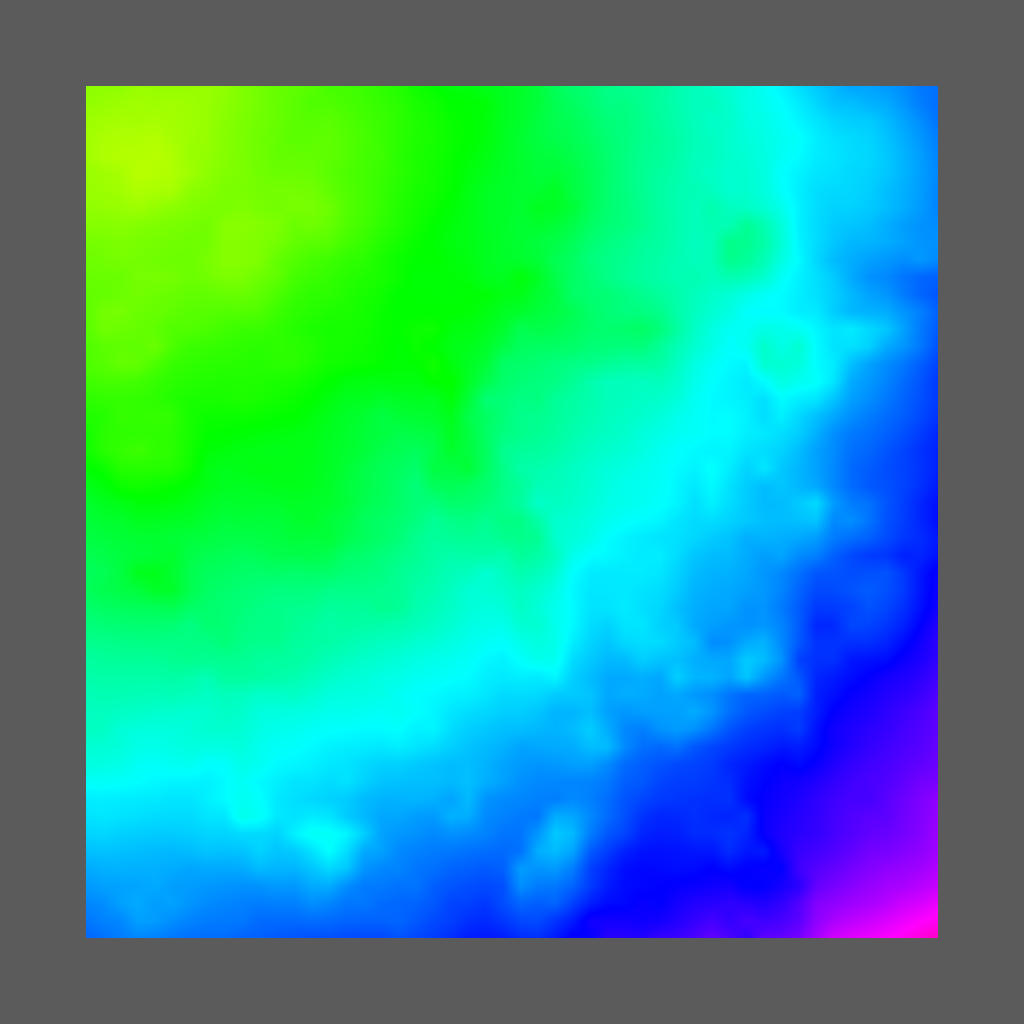
\includegraphics[width=0.16\textwidth]{../viz/num_points/H_L_MQ/1000_spheres_H_L_MQ.png}}
   \subfloat [10000] {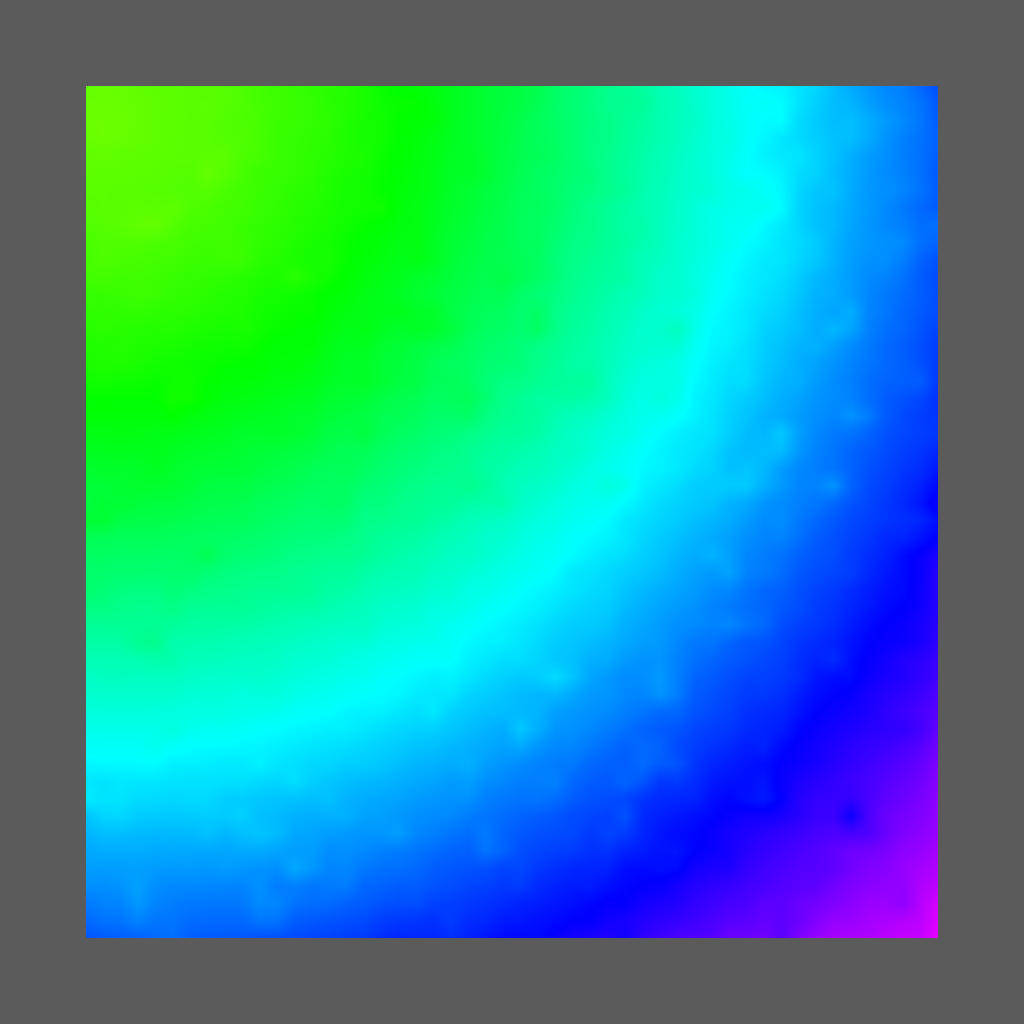
\includegraphics[width=0.16\textwidth]{../viz/num_points/H_L_MQ/10000_spheres_H_L_MQ.png}}
   \subfloat [100000] {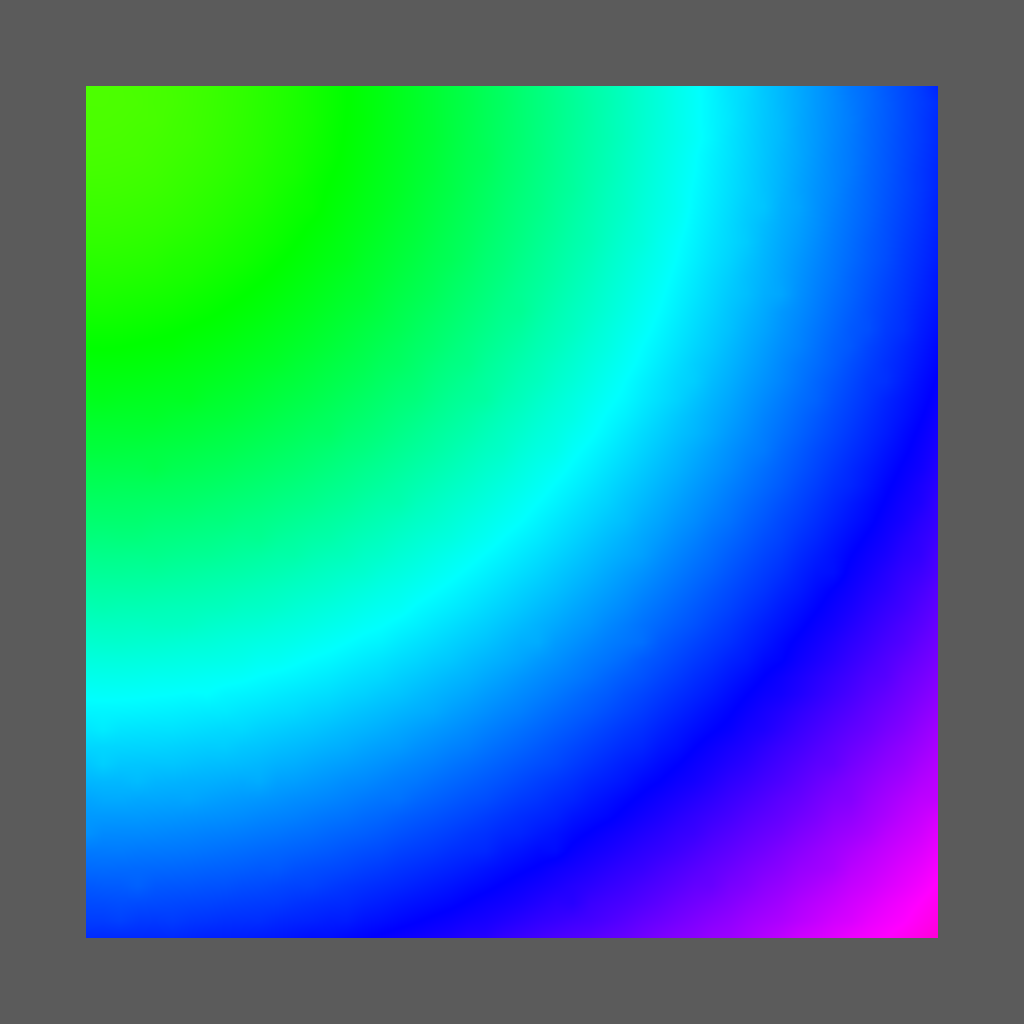
\includegraphics[width=0.16\textwidth]{../viz/num_points/H_L_MQ/100000_spheres_H_L_MQ.png}}
   \subfloat [1000000] {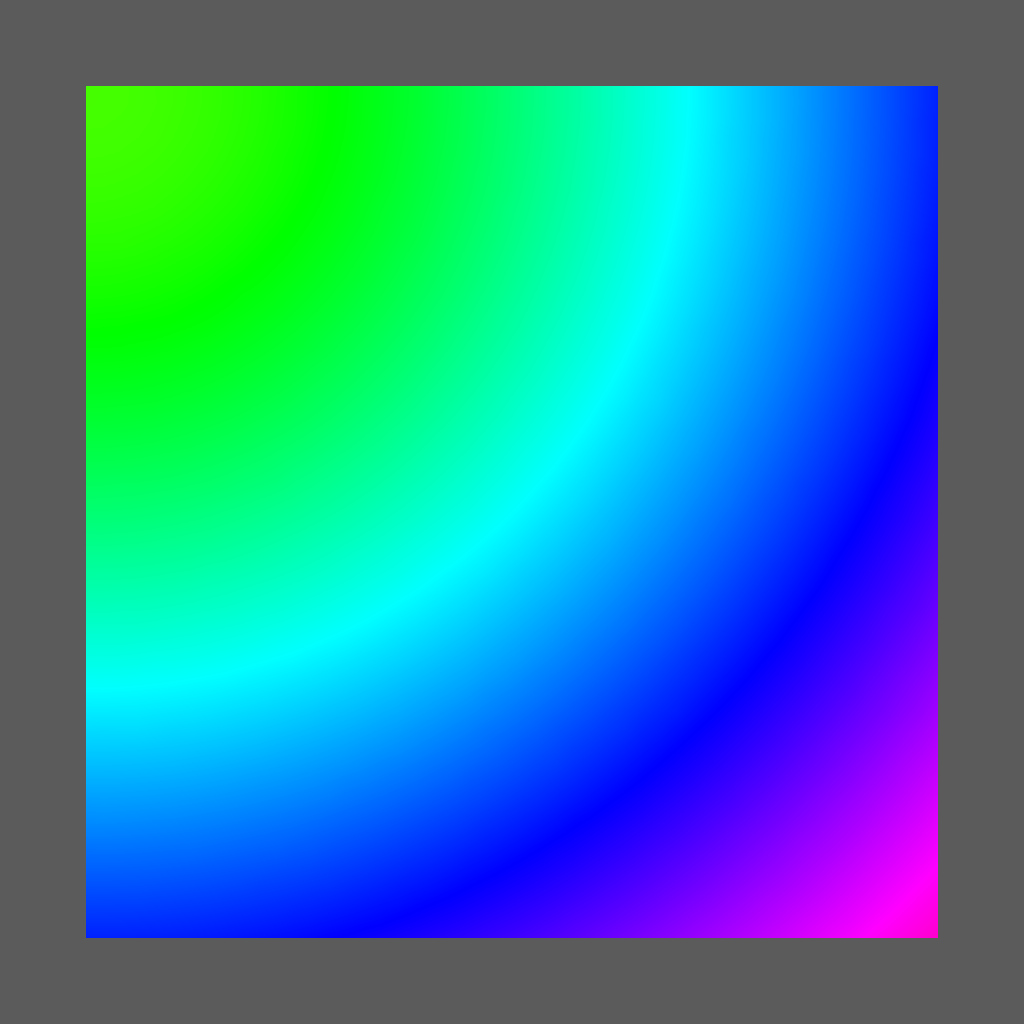
\includegraphics[width=0.16\textwidth]{../viz/num_points/H_L_MQ/1000000_spheres_H_L_MQ.png}}
   \subfloat [10000000] {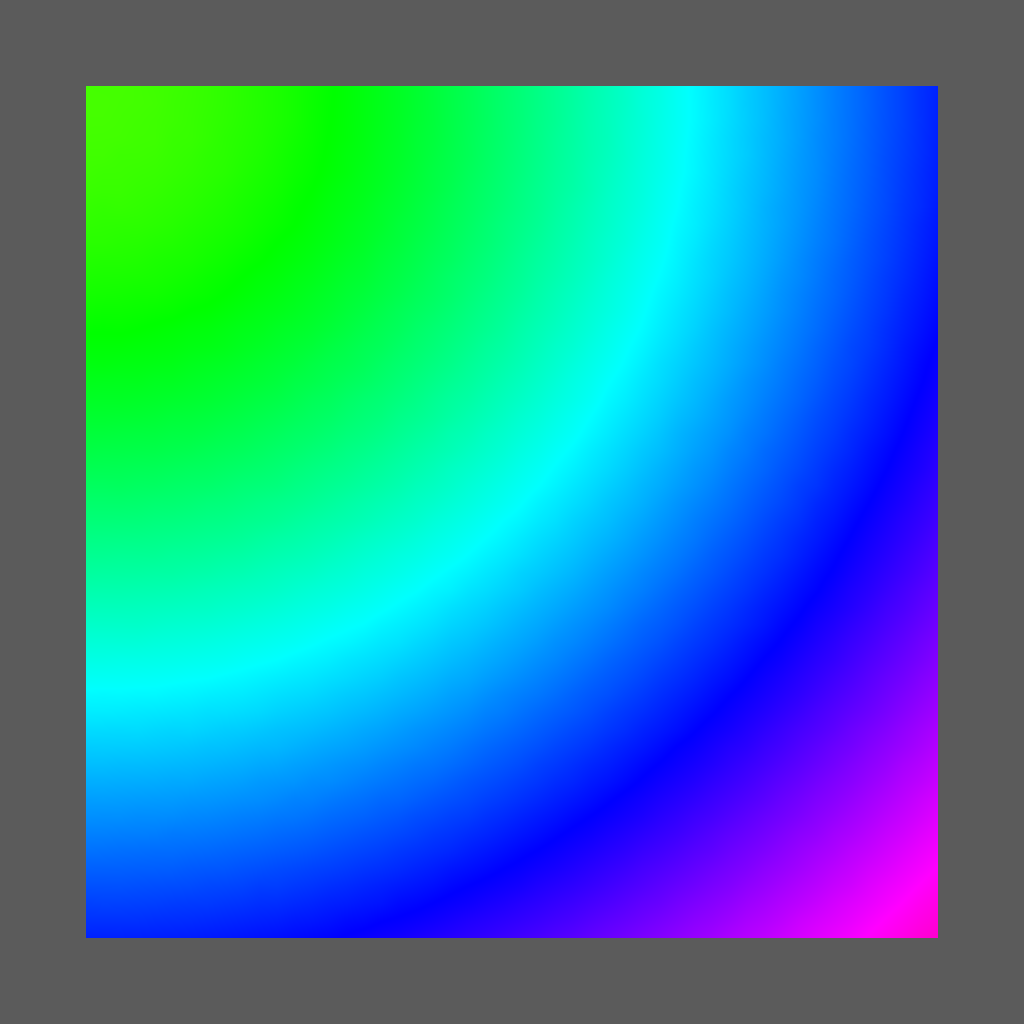
\includegraphics[width=0.16\textwidth]{../viz/num_points/H_L_MQ/10000000_spheres_H_L_MQ.png}}  
   
   \rotatebox[origin=l]{90}{G Hardy RE}	
   \subfloat [100] {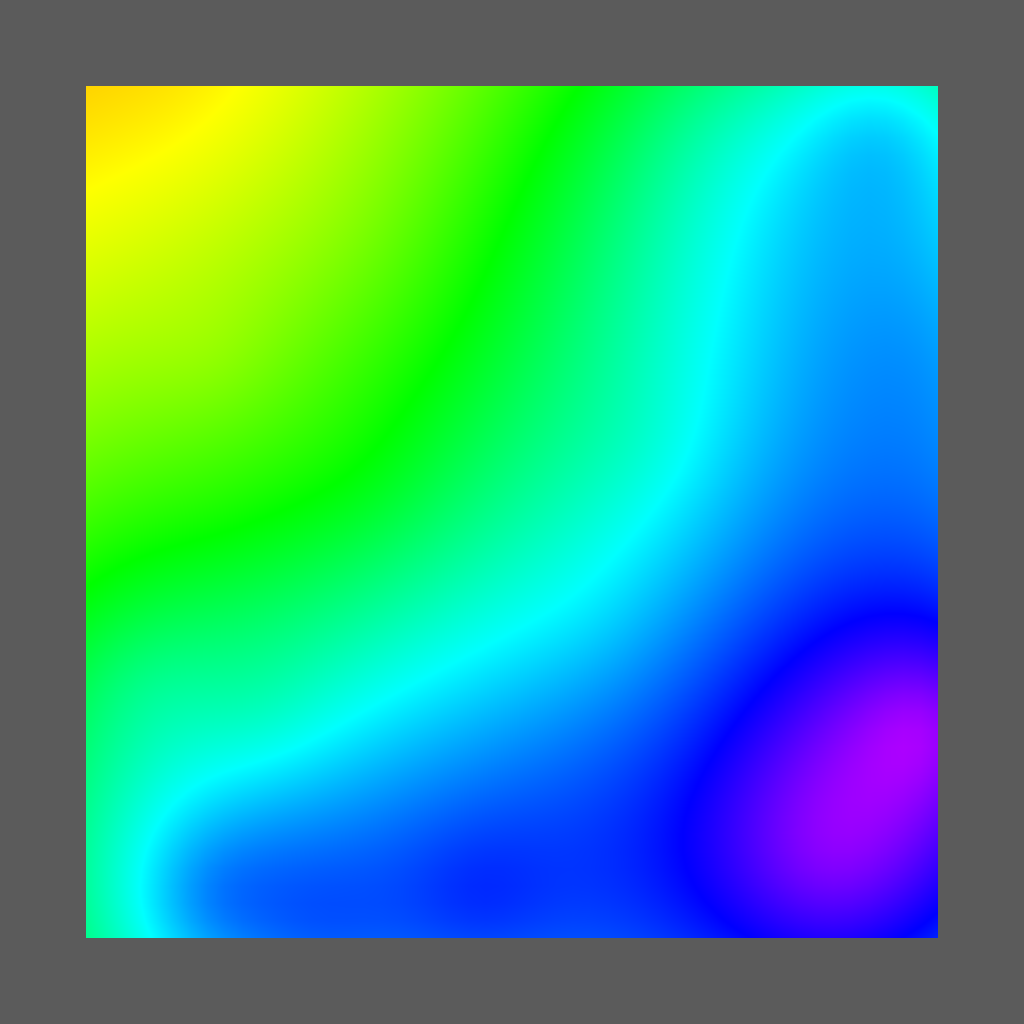
\includegraphics[width=0.16\textwidth]{../viz/num_points/H_G_RE/100_spheres_H_G_RE.png}}
   \subfloat [1000] {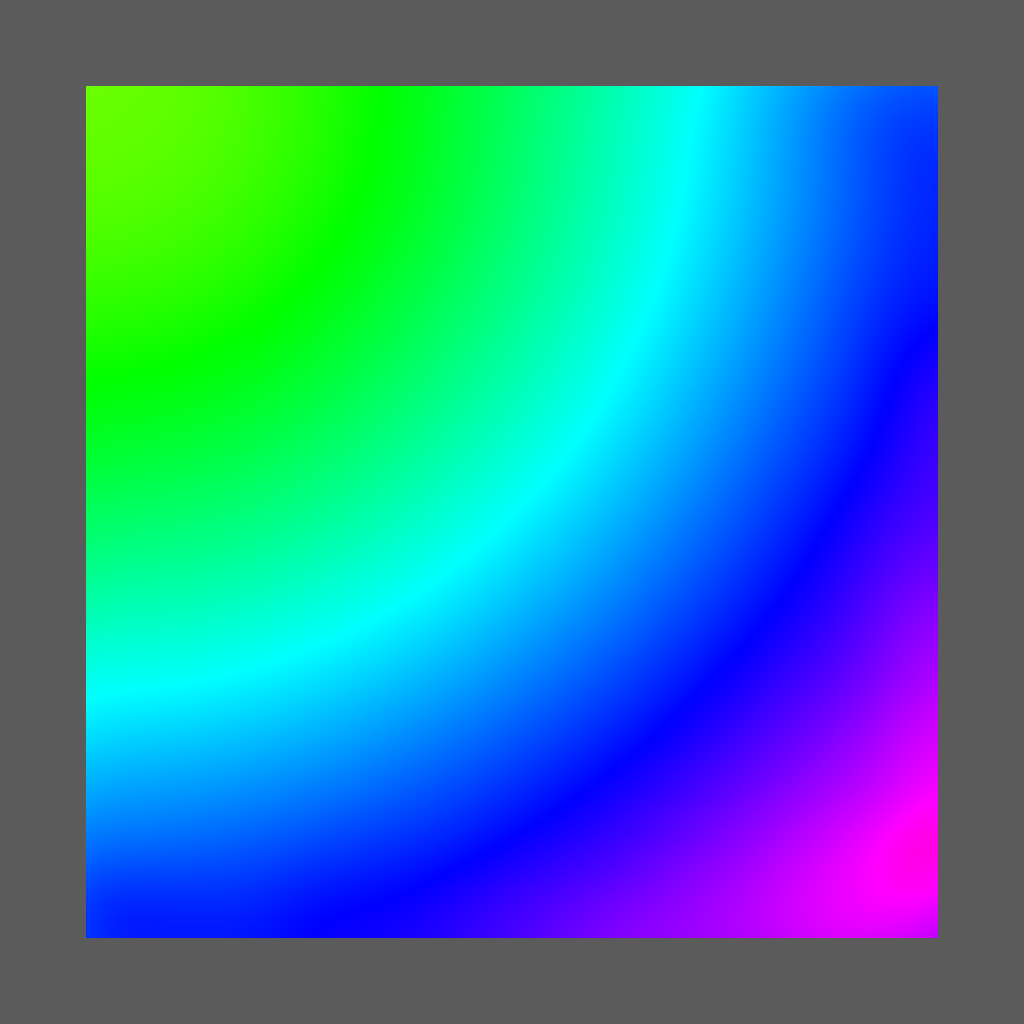
\includegraphics[width=0.16\textwidth]{../viz/num_points/H_G_RE/1000_spheres_H_G_RE.png}}
   \subfloat [10000] {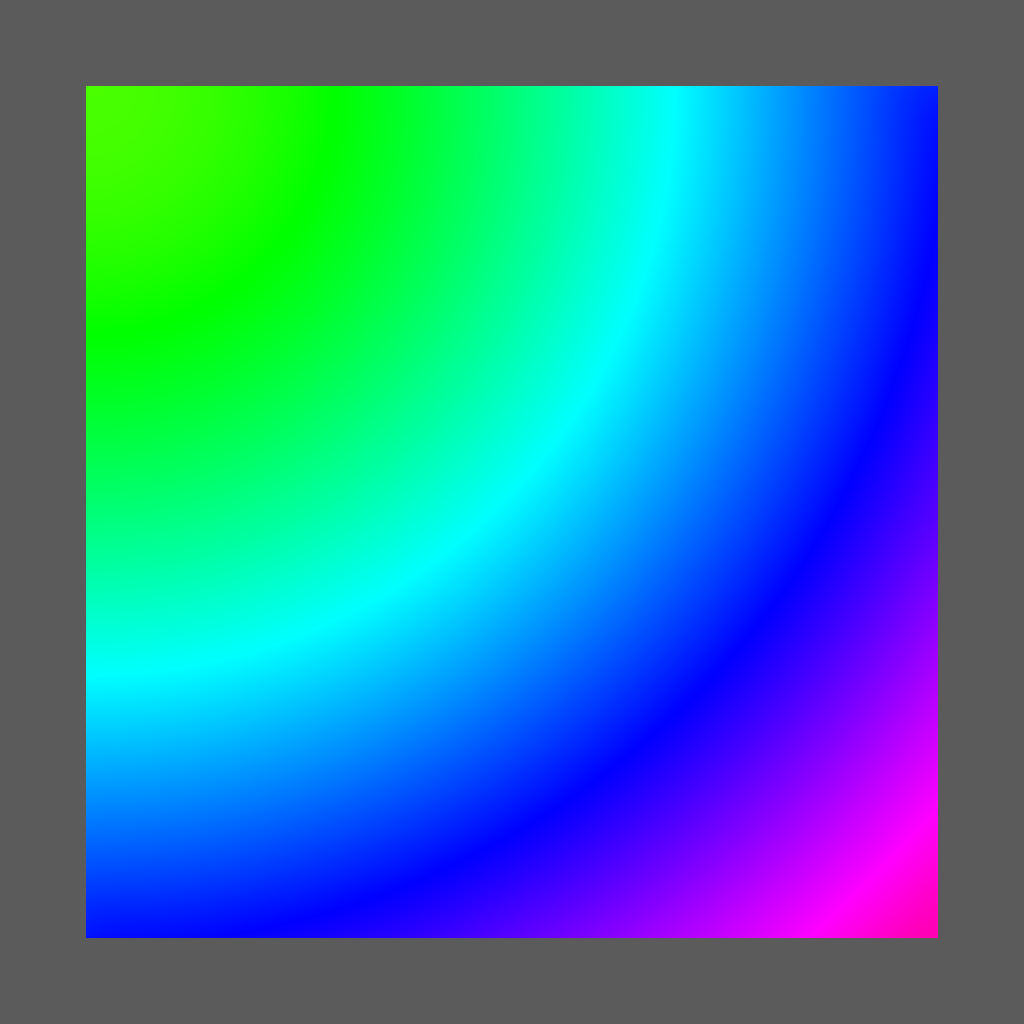
\includegraphics[width=0.16\textwidth]{../viz/num_points/H_G_RE/10000_spheres_H_G_RE.png}}
   \subfloat  {
\includegraphics[width=0.16\textwidth]{dummy.png}}
   \subfloat  {
\includegraphics[width=0.16\textwidth]{dummy.png}}
   \subfloat  {
\includegraphics[width=0.16\textwidth]{dummy.png}}   
   
   \rotatebox[origin=l]{90}{L Hardy RE}	
   \subfloat [100] {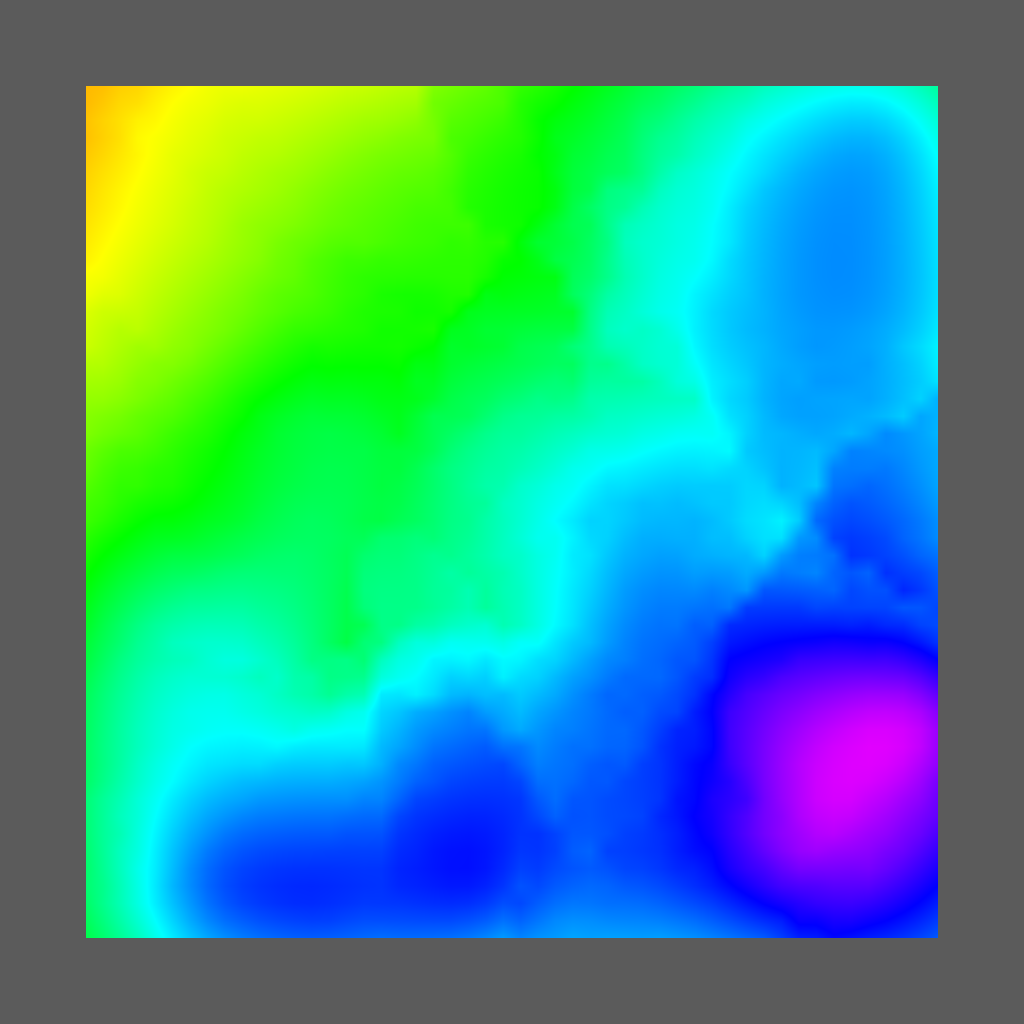
\includegraphics[width=0.16\textwidth]{../viz/num_points/H_L_RE/100_spheres_H_L_RE.png}}
   \subfloat [1000] {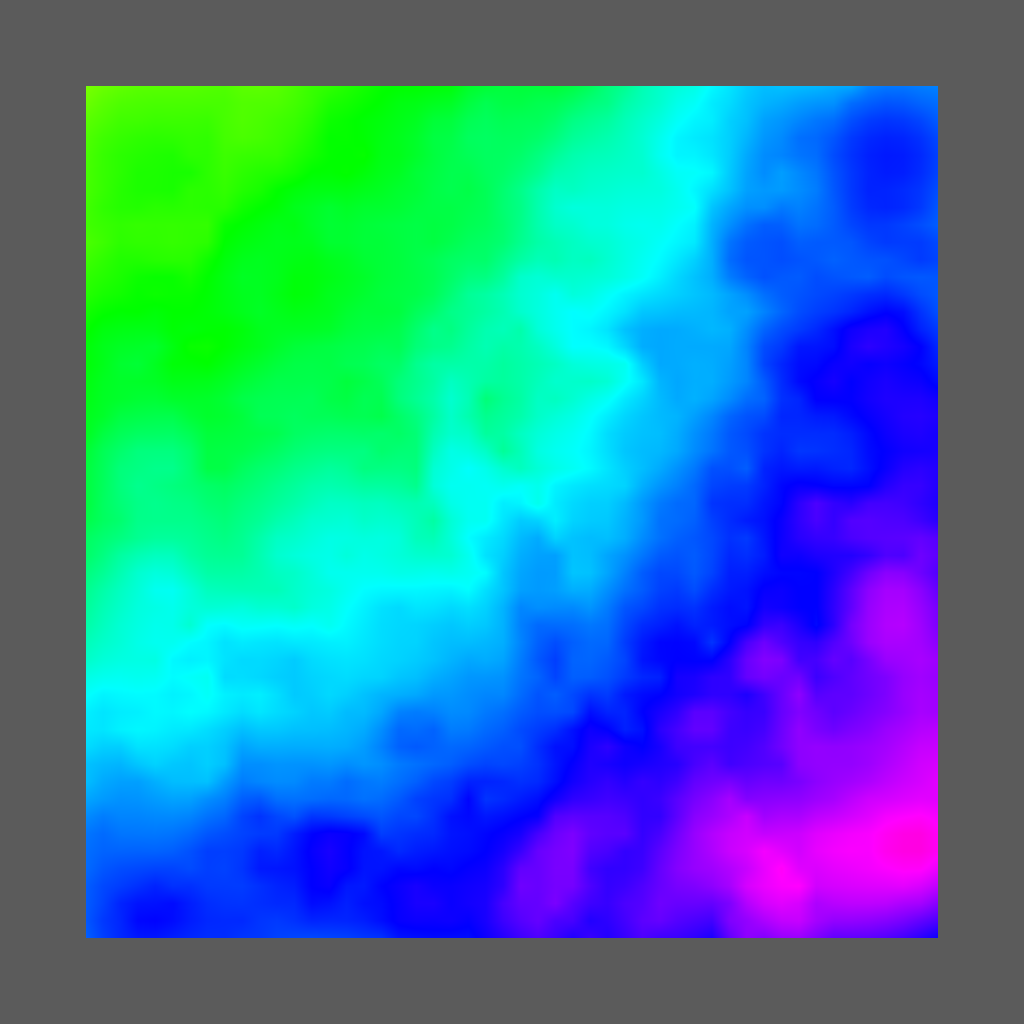
\includegraphics[width=0.16\textwidth]{../viz/num_points/H_L_RE/1000_spheres_H_L_RE.png}}
   \subfloat [10000] {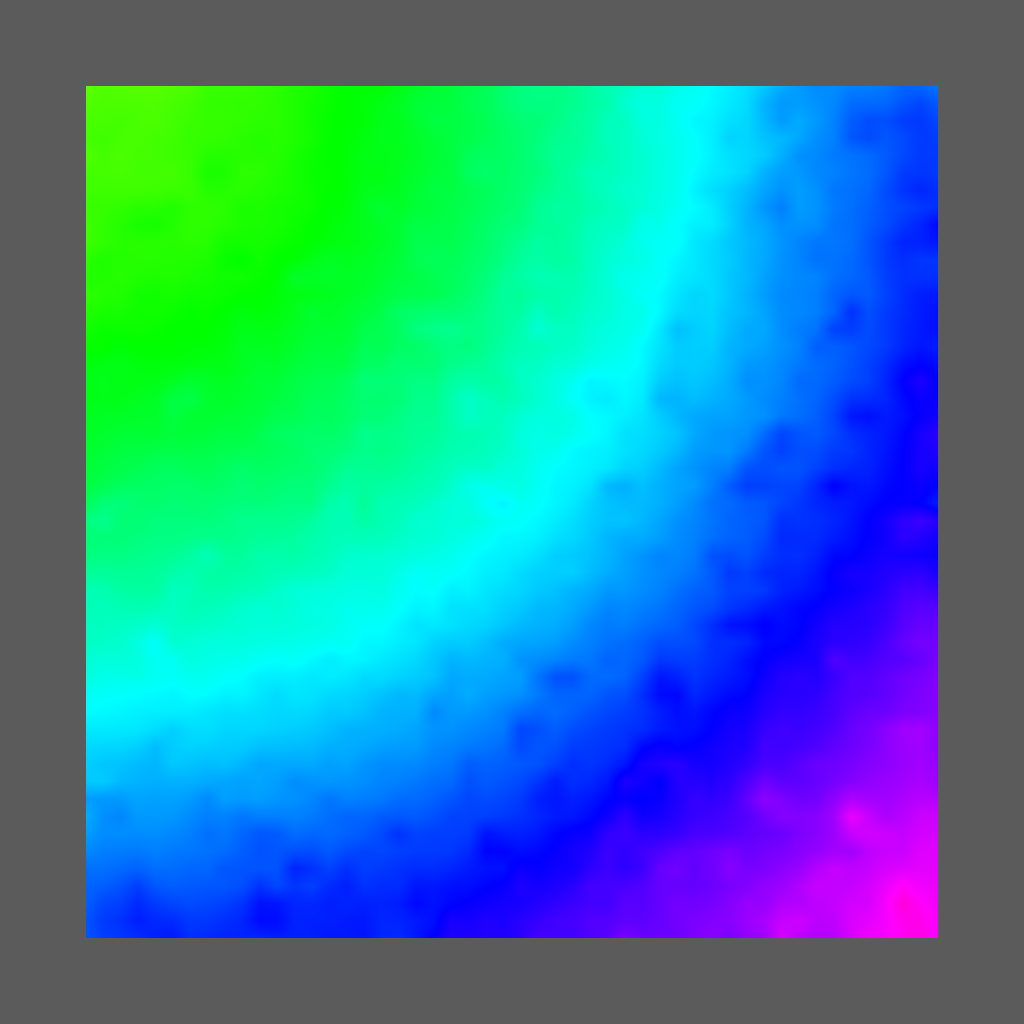
\includegraphics[width=0.16\textwidth]{../viz/num_points/H_L_RE/10000_spheres_H_L_RE.png}}
   \subfloat [100000] {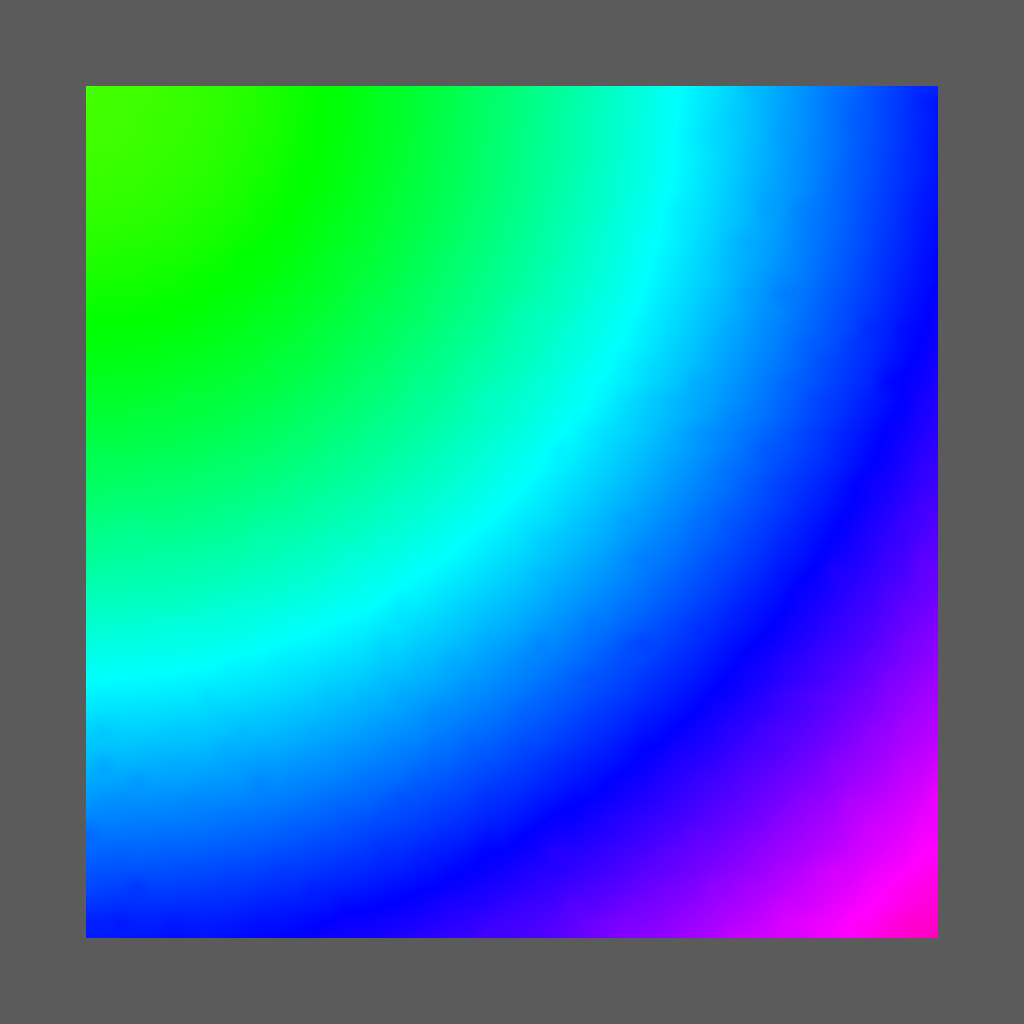
\includegraphics[width=0.16\textwidth]{../viz/num_points/H_L_RE/100000_spheres_H_L_RE.png}}
   \subfloat [1000000] {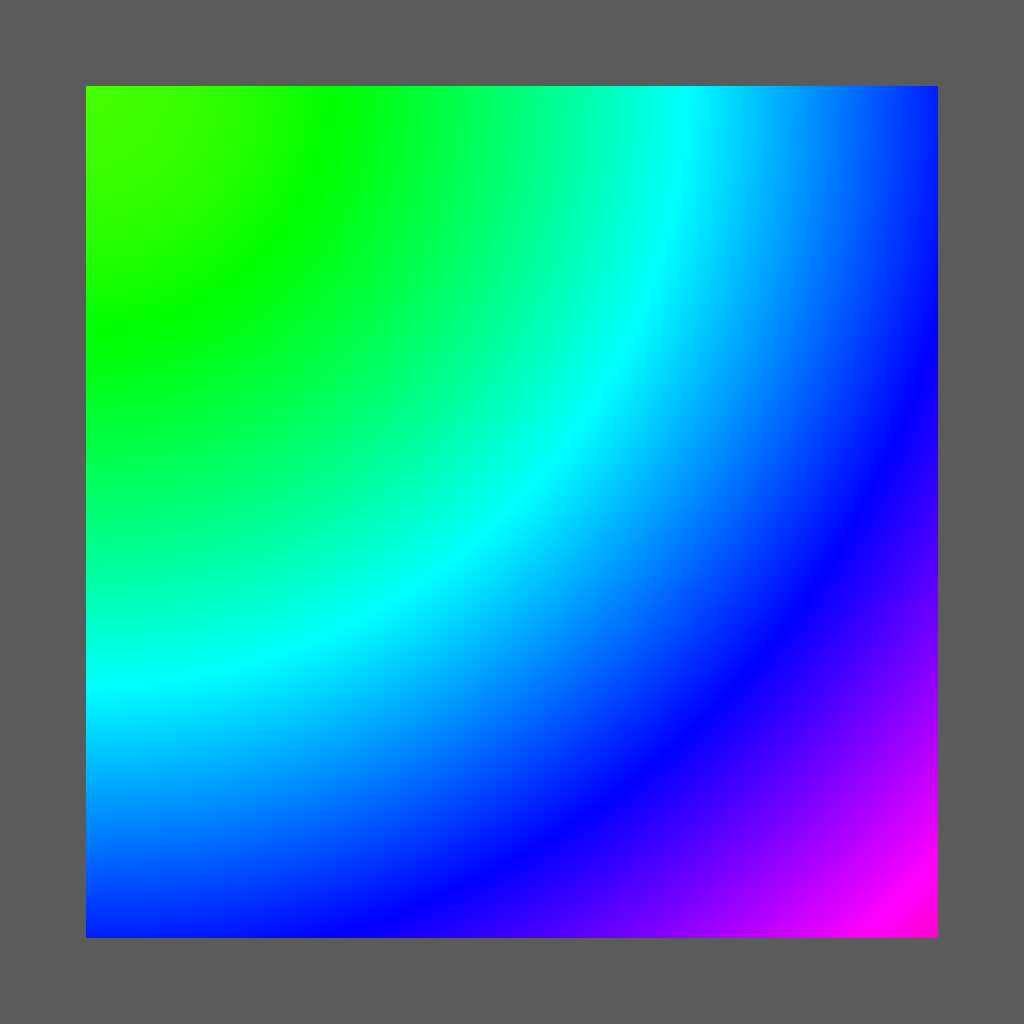
\includegraphics[width=0.16\textwidth]{../viz/num_points/H_L_RE/1000000_spheres_H_L_RE.png}}
   \subfloat [10000000] {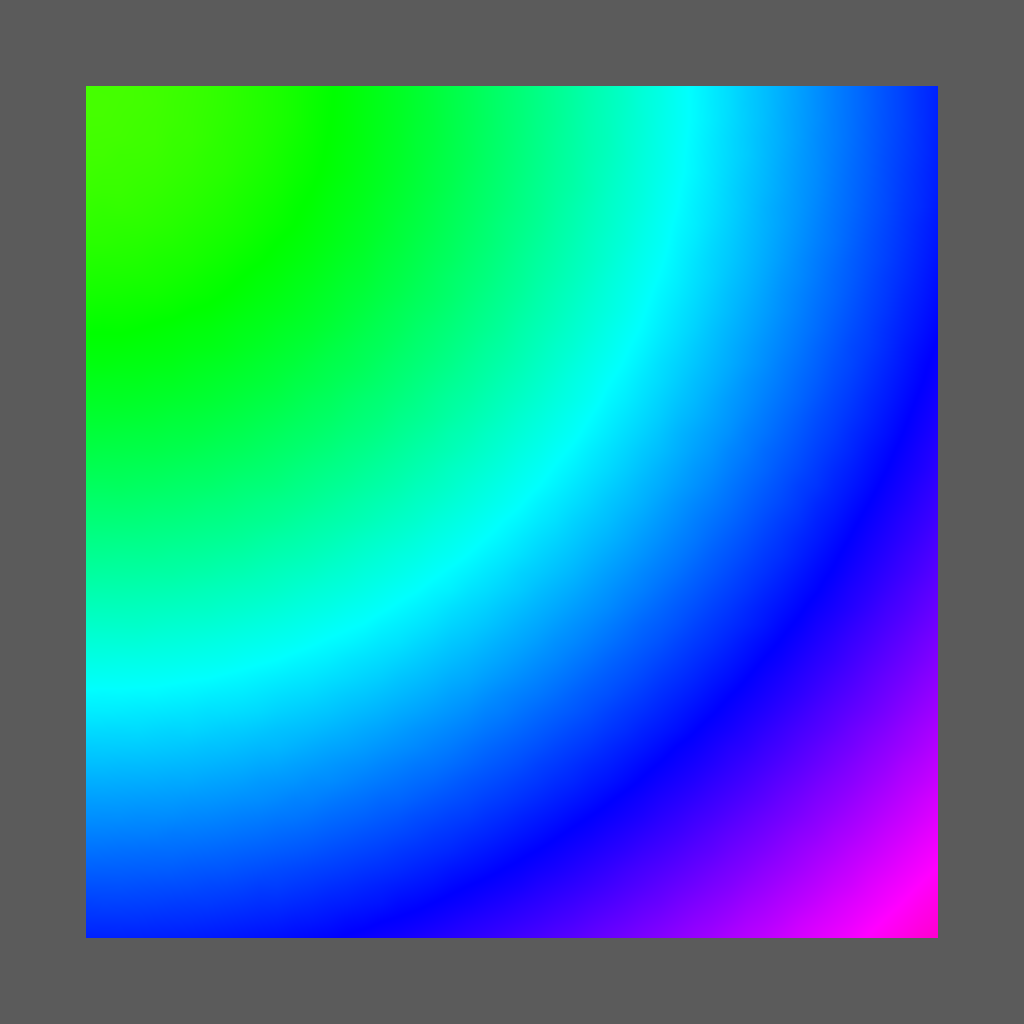
\includegraphics[width=0.16\textwidth]{../viz/num_points/H_L_RE/10000000_spheres_H_L_RE.png}} 
   
   \caption{The affect of increasing the number of the scatter data points. Here $K=10$ and $R^{2} = 0.1$.}
   \label{fig:points}
\end{figure}

%======================================================
\newpage

\begin{figure}[!tbh]
\centering     
   \rotatebox[origin=l]{90}{L Shepard's 2}
   \subfloat [3 ] {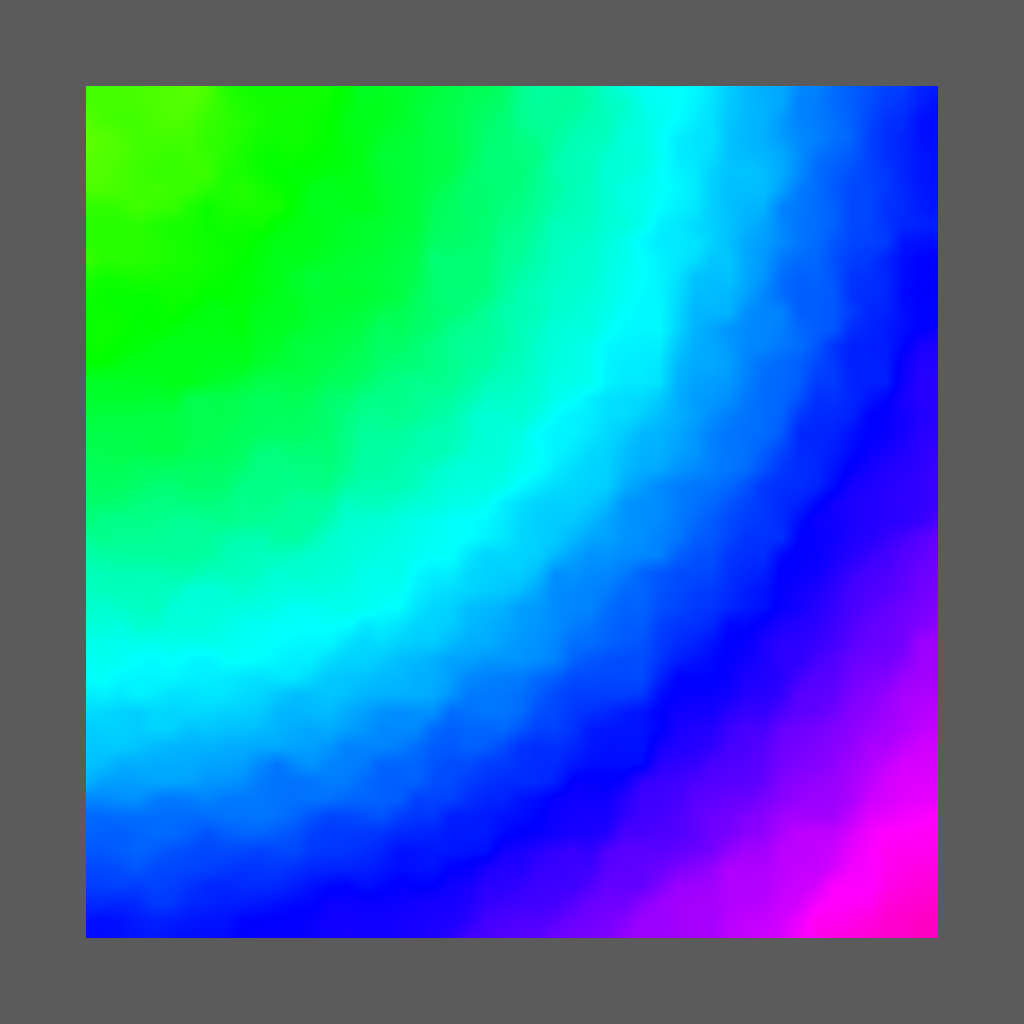
\includegraphics[width=0.138\textwidth]{../viz/kd_points/S2_L/3_spheres_S2_L.png}}
   \subfloat [6 ] {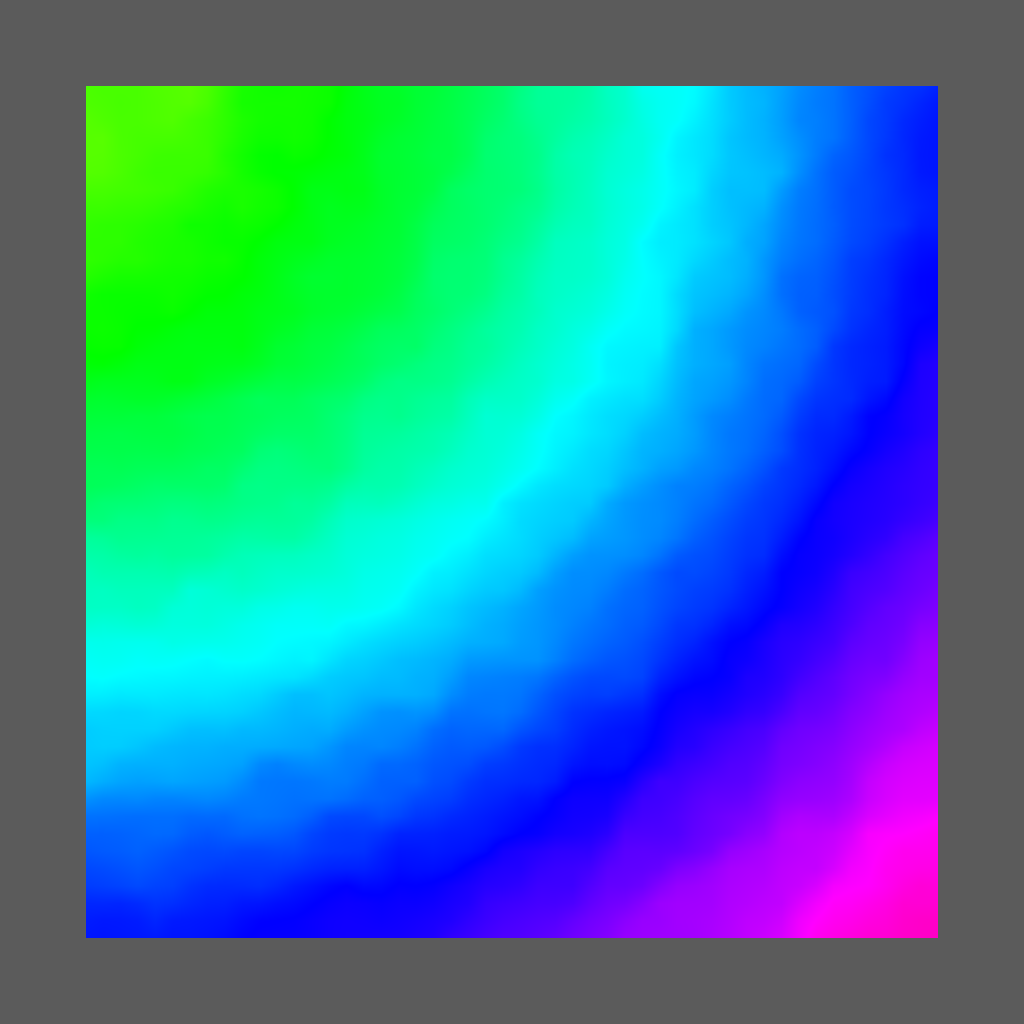
\includegraphics[width=0.138\textwidth]{../viz/kd_points/S2_L/6_spheres_S2_L.png}}
   \subfloat [9 ] {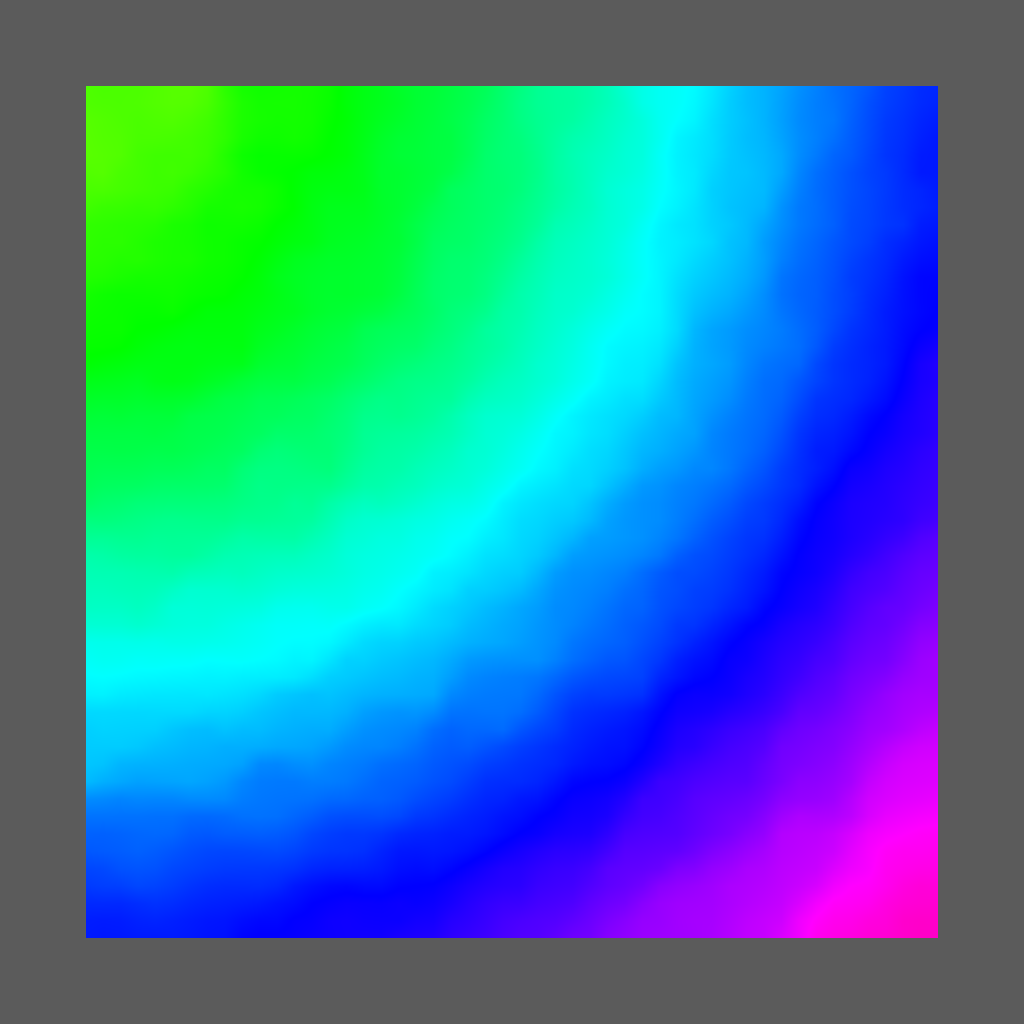
\includegraphics[width=0.138\textwidth]{../viz/kd_points/S2_L/9_spheres_S2_L.png}}
   \subfloat [12] {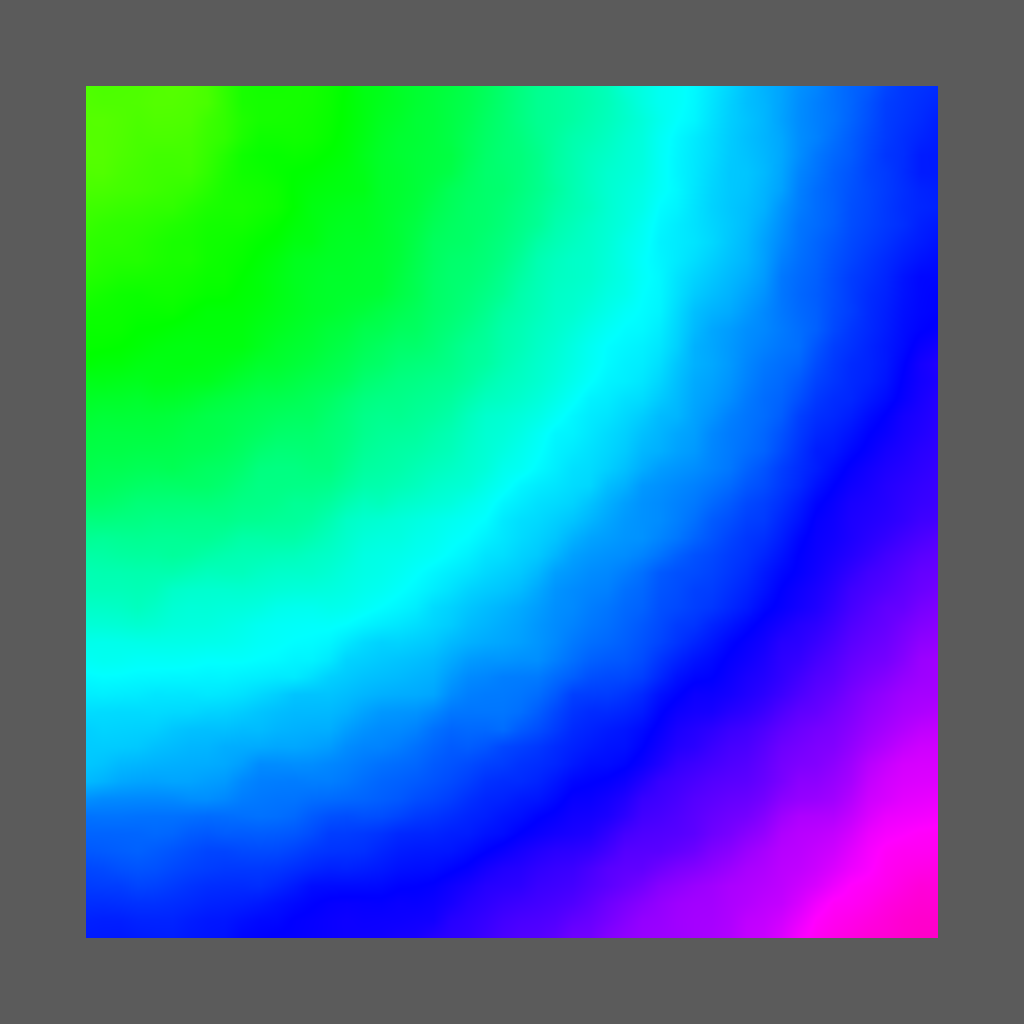
\includegraphics[width=0.138\textwidth]{../viz/kd_points/S2_L/12_spheres_S2_L.png}}
   \subfloat [15] {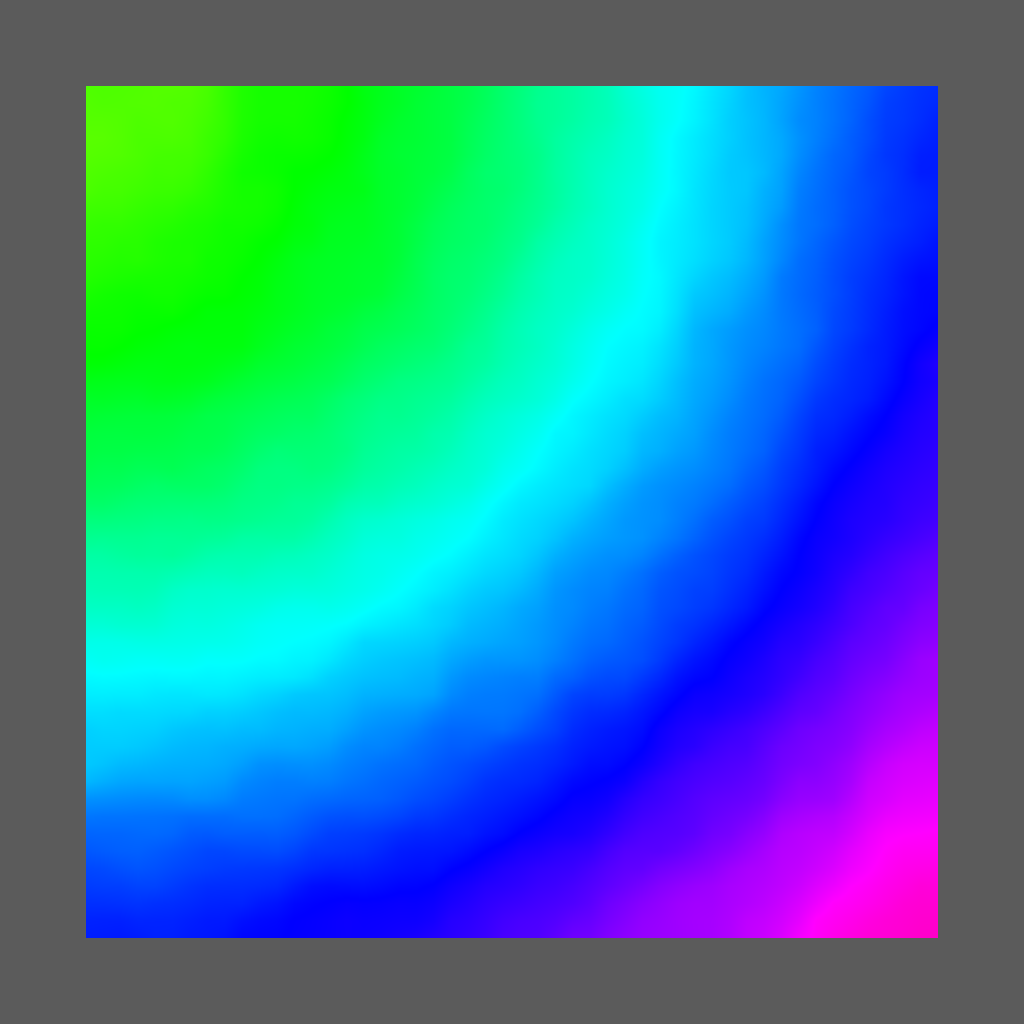
\includegraphics[width=0.138\textwidth]{../viz/kd_points/S2_L/15_spheres_S2_L.png}}
   \subfloat [18] {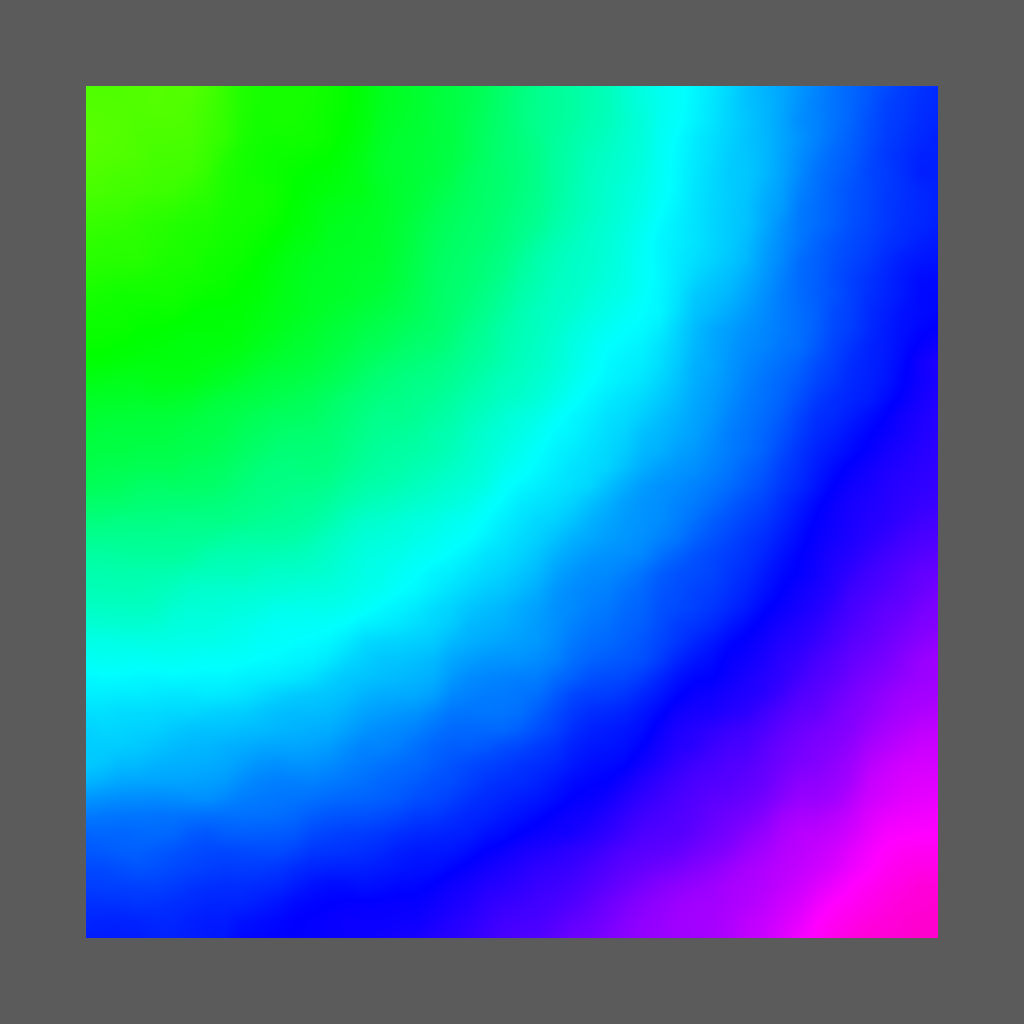
\includegraphics[width=0.138\textwidth]{../viz/kd_points/S2_L/18_spheres_S2_L.png}}   
   \subfloat [21] {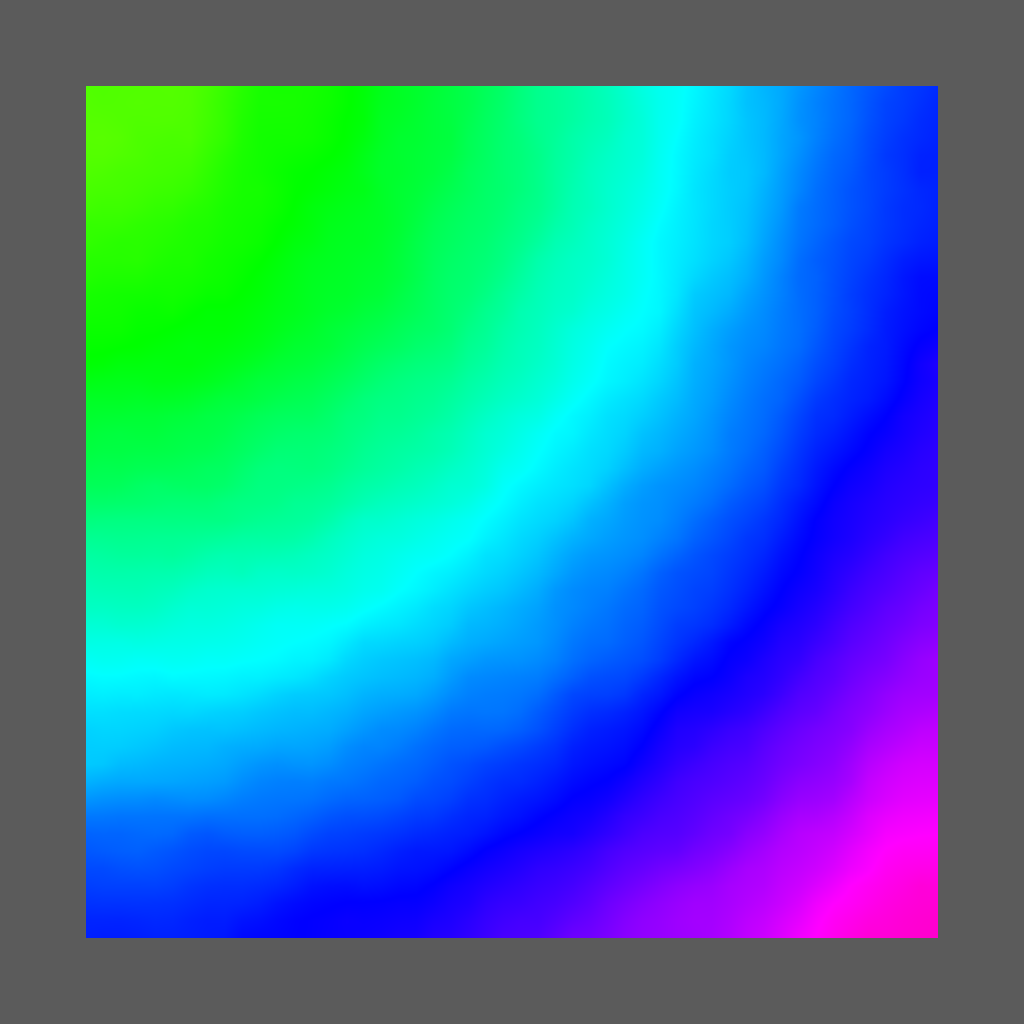
\includegraphics[width=0.138\textwidth]{../viz/kd_points/S2_L/21_spheres_S2_L.png}}
   
   \rotatebox[origin=l]{90}{L Shepard's 2}
   \subfloat [24] {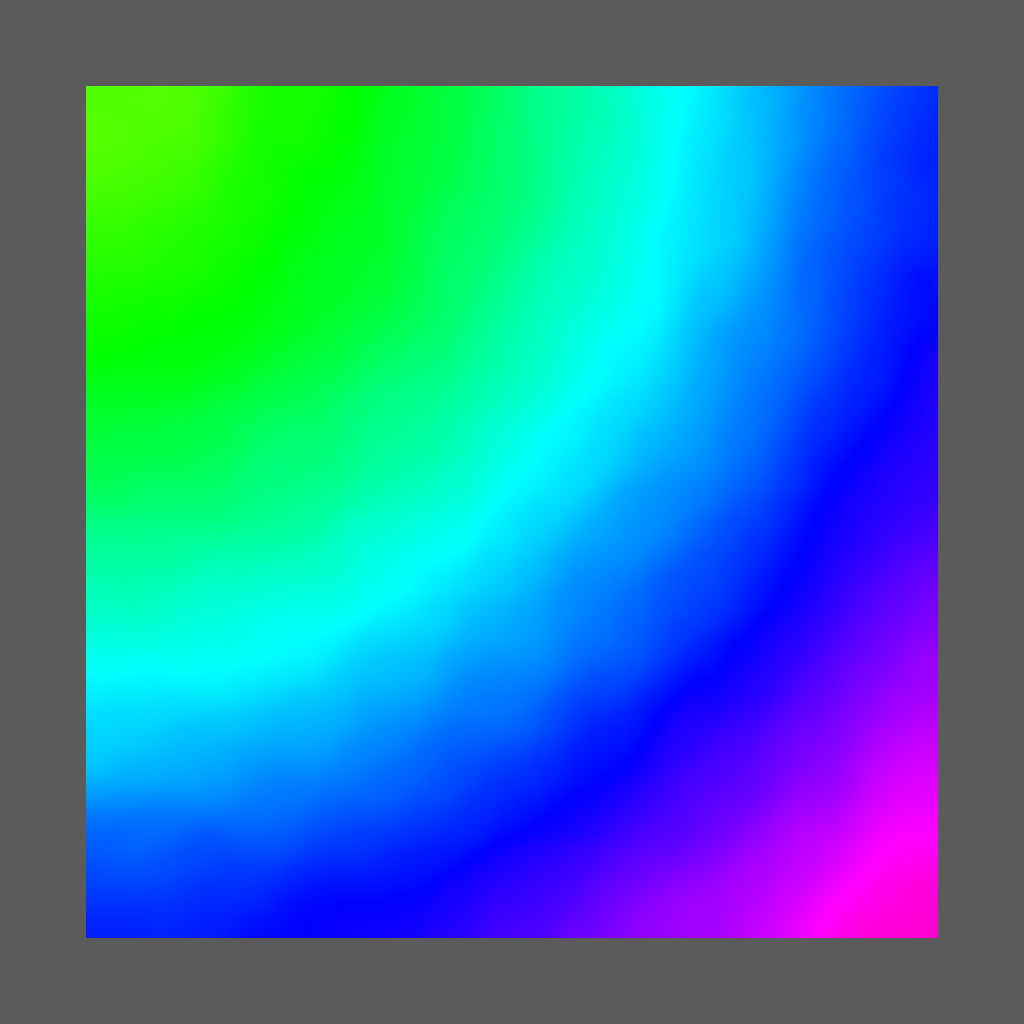
\includegraphics[width=0.138\textwidth]{../viz/kd_points/S2_L/24_spheres_S2_L.png}}
   \subfloat [27] {\includegraphics[width=0.138\textwidth]{../viz/kd_points/S2_L/27_spheres_S2_L.png}}
   \subfloat [30] {\includegraphics[width=0.138\textwidth]{../viz/kd_points/S2_L/30_spheres_S2_L.png}}
   \subfloat [33] {\includegraphics[width=0.138\textwidth]{../viz/kd_points/S2_L/33_spheres_S2_L.png}}
   \subfloat [36] {\includegraphics[width=0.138\textwidth]{../viz/kd_points/S2_L/36_spheres_S2_L.png}}
   \subfloat [39] {\includegraphics[width=0.138\textwidth]{../viz/kd_points/S2_L/39_spheres_S2_L.png}}
   \subfloat  {\includegraphics[width=0.138\textwidth]{dummy.png}}
   
   \rotatebox[origin=l]{90}{L Hardy MQ}
   \subfloat [3 ] {\includegraphics[width=0.138\textwidth]{../viz/kd_points/H_L_MQ/3_spheres_H_L_MQ.png}}
   \subfloat [6 ] {\includegraphics[width=0.138\textwidth]{../viz/kd_points/H_L_MQ/6_spheres_H_L_MQ.png}}
   \subfloat [9 ] {\includegraphics[width=0.138\textwidth]{../viz/kd_points/H_L_MQ/9_spheres_H_L_MQ.png}}
   \subfloat [12] {\includegraphics[width=0.138\textwidth]{../viz/kd_points/H_L_MQ/12_spheres_H_L_MQ.png}}
   \subfloat [15] {\includegraphics[width=0.138\textwidth]{../viz/kd_points/H_L_MQ/15_spheres_H_L_MQ.png}}
   \subfloat [18] {\includegraphics[width=0.138\textwidth]{../viz/kd_points/H_L_MQ/18_spheres_H_L_MQ.png}}
   \subfloat [21] {\includegraphics[width=0.138\textwidth]{../viz/kd_points/H_L_MQ/21_spheres_H_L_MQ.png}}
   
   \rotatebox[origin=l]{90}{L Hardy MQ}
   \subfloat [24] {\includegraphics[width=0.138\textwidth]{../viz/kd_points/H_L_MQ/24_spheres_H_L_MQ.png}}
   \subfloat [27] {\includegraphics[width=0.138\textwidth]{../viz/kd_points/H_L_MQ/27_spheres_H_L_MQ.png}}
   \subfloat [30] {\includegraphics[width=0.138\textwidth]{../viz/kd_points/H_L_MQ/30_spheres_H_L_MQ.png}}
   \subfloat [33] {\includegraphics[width=0.138\textwidth]{../viz/kd_points/H_L_MQ/33_spheres_H_L_MQ.png}}
   \subfloat [36] {\includegraphics[width=0.138\textwidth]{../viz/kd_points/H_L_MQ/36_spheres_H_L_MQ.png}}
   \subfloat [39] {\includegraphics[width=0.138\textwidth]{../viz/kd_points/H_L_MQ/39_spheres_H_L_MQ.png}}
   \subfloat  {\includegraphics[width=0.138\textwidth]{dummy.png}}
     
   \rotatebox[origin=l]{90}{L Hardy RE}
   \subfloat [3 ] {\includegraphics[width=0.138\textwidth]{../viz/kd_points/H_L_RE/3_spheres_H_L_RE.png}}
   \subfloat [6 ] {\includegraphics[width=0.138\textwidth]{../viz/kd_points/H_L_RE/6_spheres_H_L_RE.png}}
   \subfloat [9 ] {\includegraphics[width=0.138\textwidth]{../viz/kd_points/H_L_RE/9_spheres_H_L_RE.png}}
   \subfloat [12] {\includegraphics[width=0.138\textwidth]{../viz/kd_points/H_L_RE/12_spheres_H_L_RE.png}}
   \subfloat [15] {\includegraphics[width=0.138\textwidth]{../viz/kd_points/H_L_RE/15_spheres_H_L_RE.png}}
   \subfloat [18] {\includegraphics[width=0.138\textwidth]{../viz/kd_points/H_L_RE/18_spheres_H_L_RE.png}}
   \subfloat [21] {\includegraphics[width=0.138\textwidth]{../viz/kd_points/H_L_RE/21_spheres_H_L_RE.png}}
   
   \rotatebox[origin=l]{90}{L Hardy RE}
   \subfloat [24] {\includegraphics[width=0.138\textwidth]{../viz/kd_points/H_L_RE/24_spheres_H_L_RE.png}}
   \subfloat [27] {\includegraphics[width=0.138\textwidth]{../viz/kd_points/H_L_RE/27_spheres_H_L_RE.png}}
   \subfloat [30] {\includegraphics[width=0.138\textwidth]{../viz/kd_points/H_L_RE/30_spheres_H_L_RE.png}}
   \subfloat [33] {\includegraphics[width=0.138\textwidth]{../viz/kd_points/H_L_RE/33_spheres_H_L_RE.png}}
   \subfloat [36] {\includegraphics[width=0.138\textwidth]{../viz/kd_points/H_L_RE/36_spheres_H_L_RE.png}}
   \subfloat [39] {\includegraphics[width=0.138\textwidth]{../viz/kd_points/H_L_RE/39_spheres_H_L_RE.png}}   
   \subfloat  {\includegraphics[width=0.138\textwidth]{dummy.png}}
   
   \caption{The affect of changing the number of K nearest neighbors for local method. Here we used 10000 points with $R^{2}=0.1$.}
   \label{fig:k}
\end{figure}



%======================================================
\newpage

\begin{figure}[!tbh]
\centering             
   \rotatebox[origin=l]{90}{G Hardy MQ}
   \subfloat [0.01]{\includegraphics[width=0.16\textwidth]{../viz/r2/H_G_MQ/0p01_spheres_H_G_MQ.png}}
   \subfloat [0.1] {\includegraphics[width=0.16\textwidth]{../viz/r2/H_G_MQ/0p1_spheres_H_G_MQ.png}}
   \subfloat [0.2] {\includegraphics[width=0.16\textwidth]{../viz/r2/H_G_MQ/0p2_spheres_H_G_MQ.png}}
   \subfloat [0.3] {\includegraphics[width=0.16\textwidth]{../viz/r2/H_G_MQ/0p3_spheres_H_G_MQ.png}}
   \subfloat [0.4] {\includegraphics[width=0.16\textwidth]{../viz/r2/H_G_MQ/0p4_spheres_H_G_MQ.png}}
   \subfloat [0.5] {\includegraphics[width=0.16\textwidth]{../viz/r2/H_G_MQ/0p5_spheres_H_G_MQ.png}}
   
   \rotatebox[origin=l]{90}{G Hardy MQ}
   \subfloat [0.6] {\includegraphics[width=0.16\textwidth]{../viz/r2/H_G_MQ/0p6_spheres_H_G_MQ.png}}
   \subfloat [0.7] {\includegraphics[width=0.16\textwidth]{../viz/r2/H_G_MQ/0p7_spheres_H_G_MQ.png}}
   \subfloat [0.8] {\includegraphics[width=0.16\textwidth]{../viz/r2/H_G_MQ/0p8_spheres_H_G_MQ.png}}
   \subfloat [0.9] {\includegraphics[width=0.16\textwidth]{../viz/r2/H_G_MQ/0p9_spheres_H_G_MQ.png}}
   \subfloat [0.99]{\includegraphics[width=0.16\textwidth]{../viz/r2/H_G_MQ/0p99_spheres_H_G_MQ.png}}
   \subfloat  {\includegraphics[width=0.16\textwidth]{dummy.png}}
   
   \rotatebox[origin=l]{90}{L Hardy MQ}
   \subfloat [0.01]{\includegraphics[width=0.16\textwidth]{../viz/r2/H_L_MQ/0p01_spheres_H_L_MQ.png}}
   \subfloat [0.1] {\includegraphics[width=0.16\textwidth]{../viz/r2/H_L_MQ/0p1_spheres_H_L_MQ.png}}
   \subfloat [0.2] {\includegraphics[width=0.16\textwidth]{../viz/r2/H_L_MQ/0p2_spheres_H_L_MQ.png}}
   \subfloat [0.3] {\includegraphics[width=0.16\textwidth]{../viz/r2/H_L_MQ/0p3_spheres_H_L_MQ.png}}
   \subfloat [0.4] {\includegraphics[width=0.16\textwidth]{../viz/r2/H_L_MQ/0p4_spheres_H_L_MQ.png}}
   \subfloat [0.5] {\includegraphics[width=0.16\textwidth]{../viz/r2/H_L_MQ/0p5_spheres_H_L_MQ.png}}
   
   \rotatebox[origin=l]{90}{L Hardy MQ}
   \subfloat [0.6] {\includegraphics[width=0.16\textwidth]{../viz/r2/H_L_MQ/0p6_spheres_H_L_MQ.png}}
   \subfloat [0.7] {\includegraphics[width=0.16\textwidth]{../viz/r2/H_L_MQ/0p7_spheres_H_L_MQ.png}}
   \subfloat [0.8] {\includegraphics[width=0.16\textwidth]{../viz/r2/H_L_MQ/0p8_spheres_H_L_MQ.png}}
   \subfloat [0.9] {\includegraphics[width=0.16\textwidth]{../viz/r2/H_L_MQ/0p9_spheres_H_L_MQ.png}}
   \subfloat [0.99]{\includegraphics[width=0.16\textwidth]{../viz/r2/H_L_MQ/0p99_spheres_H_L_MQ.png}}
   \subfloat  {\includegraphics[width=0.16\textwidth]{dummy.png}}
   
   \rotatebox[origin=l]{90}{G Hardy RE}
   \subfloat [0.01]{\includegraphics[width=0.16\textwidth]{../viz/r2/H_G_RE/0p01_spheres_H_G_RE.png}}
   \subfloat [0.1] {\includegraphics[width=0.16\textwidth]{../viz/r2/H_G_RE/0p1_spheres_H_G_RE.png}}
   \subfloat [0.2] {\includegraphics[width=0.16\textwidth]{../viz/r2/H_G_RE/0p2_spheres_H_G_RE.png}}
   \subfloat [0.3] {\includegraphics[width=0.16\textwidth]{../viz/r2/H_G_RE/0p3_spheres_H_G_RE.png}}
   \subfloat [0.4] {\includegraphics[width=0.16\textwidth]{../viz/r2/H_G_RE/0p4_spheres_H_G_RE.png}}
   \subfloat [0.5] {\includegraphics[width=0.16\textwidth]{../viz/r2/H_G_RE/0p5_spheres_H_G_RE.png}}
   
   \rotatebox[origin=l]{90}{G Hardy RE}
   \subfloat [0.6] {\includegraphics[width=0.16\textwidth]{../viz/r2/H_G_RE/0p6_spheres_H_G_RE.png}}
   \subfloat [0.7] {\includegraphics[width=0.16\textwidth]{../viz/r2/H_G_RE/0p7_spheres_H_G_RE.png}}
   \subfloat [0.8] {\includegraphics[width=0.16\textwidth]{../viz/r2/H_G_RE/0p8_spheres_H_G_RE.png}}
   \subfloat [0.9] {\includegraphics[width=0.16\textwidth]{../viz/r2/H_G_RE/0p9_spheres_H_G_RE.png}}
   \subfloat [0.99]{\includegraphics[width=0.16\textwidth]{../viz/r2/H_G_RE/0p99_spheres_H_G_RE.png}}
   \subfloat  {\includegraphics[width=0.16\textwidth]{dummy.png}}
   
   \caption{The affect of $R^{2}$ factor in Hardy's methods. Here we used 10000 points with $K=10$.}
   \label{fig:r2}
\end{figure}

\newpage
\makeatletter
\setlength{\@fptop}{0pt}
\makeatother
\begin{figure}[t!]
\centering        
   \rotatebox[origin=l]{90}{L Hardy RE}
   \subfloat [0.01]{\includegraphics[width=0.16\textwidth]{../viz/r2/H_L_RE/0p01_spheres_H_L_RE.png}}
   \subfloat [0.1] {\includegraphics[width=0.16\textwidth]{../viz/r2/H_L_RE/0p1_spheres_H_L_RE.png}}
   \subfloat [0.2] {\includegraphics[width=0.16\textwidth]{../viz/r2/H_L_RE/0p2_spheres_H_L_RE.png}}
   \subfloat [0.3] {\includegraphics[width=0.16\textwidth]{../viz/r2/H_L_RE/0p3_spheres_H_L_RE.png}}
   \subfloat [0.4] {\includegraphics[width=0.16\textwidth]{../viz/r2/H_L_RE/0p4_spheres_H_L_RE.png}}
   \subfloat [0.5] {\includegraphics[width=0.16\textwidth]{../viz/r2/H_L_RE/0p5_spheres_H_L_RE.png}}
   
   \rotatebox[origin=l]{90}{L Hardy RE}
   \subfloat [0.6] {\includegraphics[width=0.16\textwidth]{../viz/r2/H_L_RE/0p6_spheres_H_L_RE.png}}
   \subfloat [0.7] {\includegraphics[width=0.16\textwidth]{../viz/r2/H_L_RE/0p7_spheres_H_L_RE.png}}
   \subfloat [0.8] {\includegraphics[width=0.16\textwidth]{../viz/r2/H_L_RE/0p8_spheres_H_L_RE.png}}
   \subfloat [0.9] {\includegraphics[width=0.16\textwidth]{../viz/r2/H_L_RE/0p9_spheres_H_L_RE.png}}
   \subfloat [0.99]{\includegraphics[width=0.16\textwidth]{../viz/r2/H_L_RE/0p99_spheres_H_L_RE.png}}   
   \subfloat  {\includegraphics[width=0.16\textwidth]{dummy.png}}
   \caption{The affect of $R^{2}$ factor in Hardy's methods. Here we used 10000 points with $K=10$.}
   \label{fig:r2}
\end{figure}



\bibliography{../mybib}
\bibliographystyle{plain}
\end{document}